\documentclass[../main.tex]{subfiles}
	% THE RASPBERRY PI AND THE TEST BED
\begin{document}

Talk about the RPi and test bed.

%%%%%%%%%%%%%%%%%%%%%%%%%%%%%%%%%%%%%%%%%%%%%%%%%%%%%%%%%%%%%%%%%%%%%%%%%%%%%%%%%%%%%%%%%%%%%%%%%%%%%%%%%%%%%%%%%%%%%%%%%%%%%%%%%%

\section{Fundamentals}

The Raspberry Pi is a simple, affordable ARM-based computing module. It has, which can interface\\

It is run using a Linux-based operating system called Raspbian which is available for download from the Raspberry Pi official website \ref{web_Raspbian} \ref{web_Rasp}.\\

\todo[inline,color=blue!20]{Raspberry Pi Fundamentals}

\begin{figure}[ht]
	\centering
	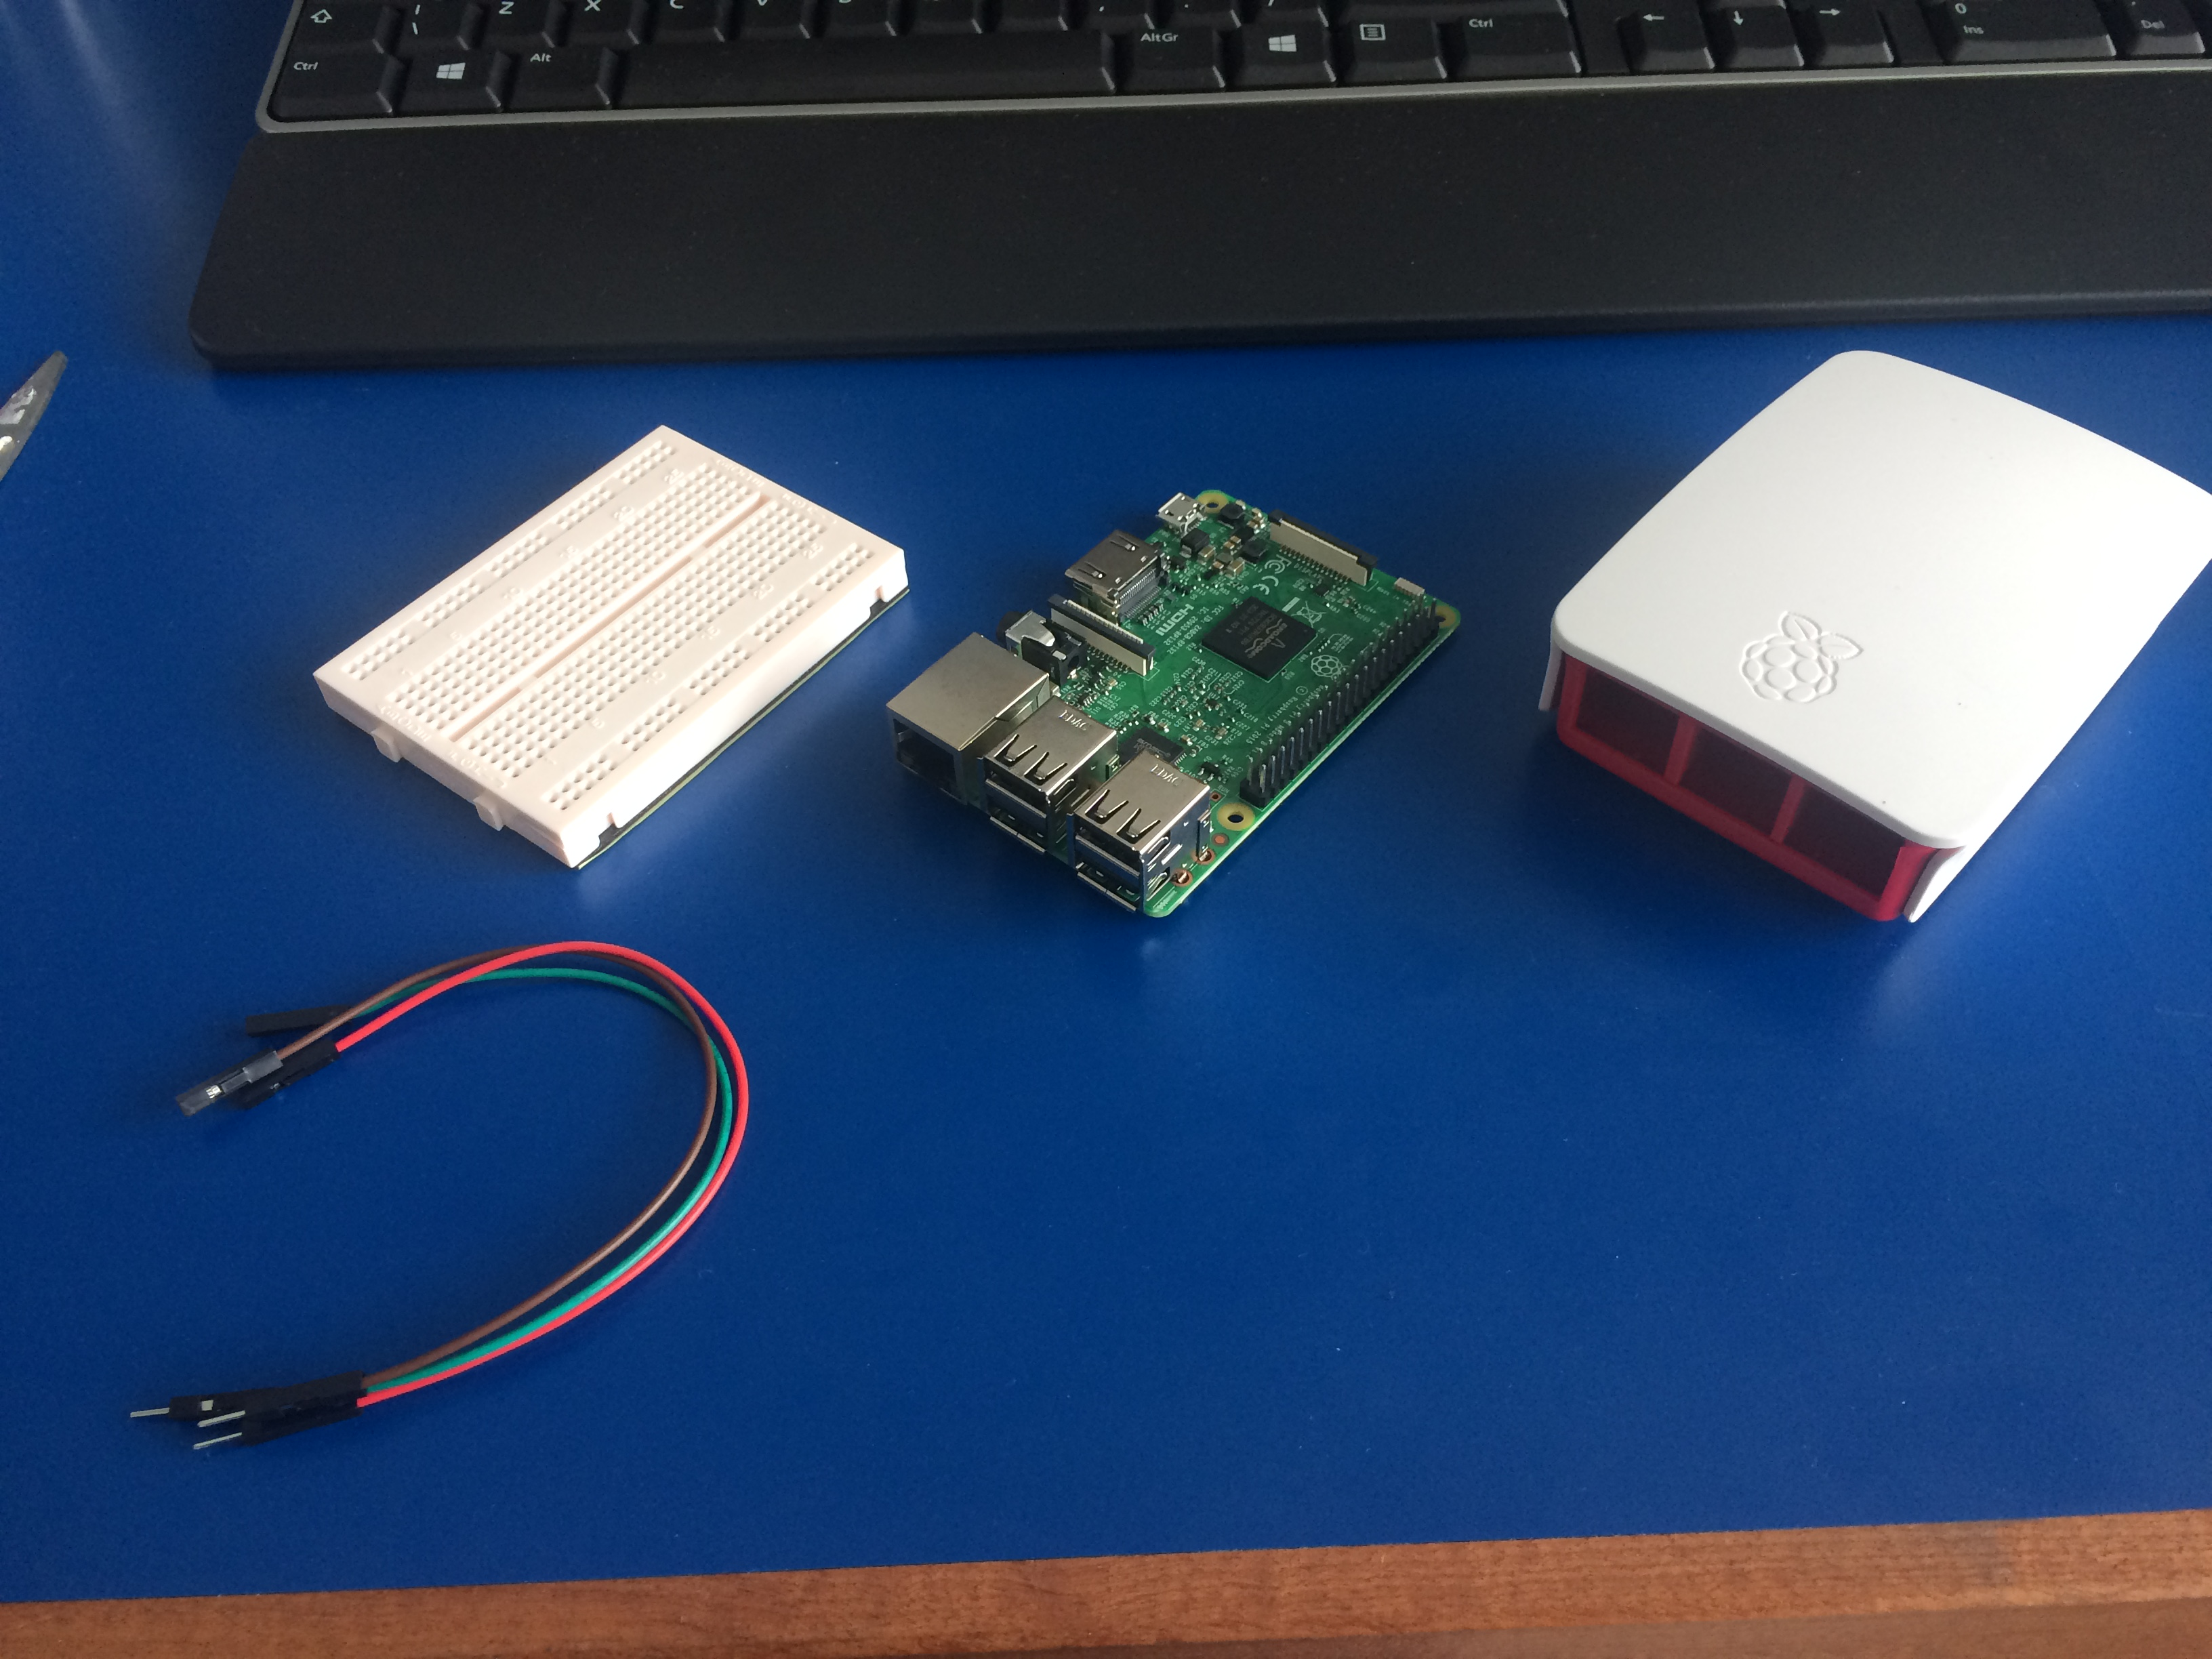
\includegraphics[width=0.6\textwidth]{Raspberry_Pi.jpg}
	\caption{The Raspberry Pi}
	%\label{fig_}
\end{figure}

\subsection{Setting up the Raspberry Pi}

The Raspberry Pi can be interfaced with in a number of ways, but first it needs to be set up with its operating system on the SD card \ref{web_Setup Raspbian}.
\todo[inline,color=blue!20]{MISSING REFERENCE - How to setup Raspbian https://hackernoon.com/raspberry-pi-headless-install-462ccabd75d0}
Raspbian can be accessed via the command line - typing in commands - or through an X Window similar to Windows OS.
Either of these options can be used by connecting a screen, keyboard and mouse to the Pi, but this is not always available, so it is useful to have Secure Shell (SSH) set up for the command line, and Virtual Network Computing (VNC) for the X Window.
When actually using both Raspberry Pis in the test bed, both of them will be running in command line mode as this saves resources, although during development, VNC or a screen using the X Window is much easier.
In the test bed the Transmitter Pi will be connected to a screen and peripherals in command line, and then it will start the Receiver via SSH, which will run headless (without a screen or control peripherals) and receive the data, process and output it, and store information about the run in a log file which can be accessed later or again through SSH.\\

Once the operating system is written to the SD card, SSH can be enabled by creating an empty file 'ssh' in the main portion of the card before putting it in the Raspberry Pi.
Now an Ethernet cable can be connected from a computer to the Pi and it can be logged into.
A program such as PuTTY for Windows can be used, with "pi@raspberrypi.local" as the host name so the IP address isn't needed.
The standard login is "username: pi" and "password: raspberry".
\todo[inline,color=green!40]{Inline code reference should look like inline code}
The command "sudo raspi-config" accesses the configuration settings where the file system can be expanded to the whole SD card, and other utilities such as Wi-Fi and VNC can be turned on.
Again, these can be turned off when using the final test bed to improve performance of the devices.
Once the Pi is connected to Wi-Fi and the IP address is known, it can be accessed remotely via the free RealVNC VNC Viewer \ref{web_RealVNC Viewer} and the X Window can be started with the command "startx" if it isn't already set to open the X Window on startup in the configuration settings.
\todo[inline,color=blue!20]{MISSING REFERENCE - https://www.realvnc.com/en/connect/download/viewer/}
This access can be made permanent by setting the Pi to have a static IP address or with a free RealVNC account which lets it be accessed independent of the IP address.\\

With full control of the Pi, all that is needed is to download all of the libraries and software used by the test bed and clone the GitHub repository with its code.
The Python version used is 3.x.x.
\todo[inline]{Find python version of Pis}
and as the Raspberry Pi has Python 2 and 3, pip - the Python package manager - is called as pip3 for python3.
Any dependencies not in this list give clear instructions how to be downloaded when this is run line by line.\\

\todo[inline,color=green!40]{Create new format (and inline for above) called "shell"}
\todo[inline]{Include matplotlib if used in the end - ALSO INCLUDE REFERENCES TO ALL LIBRARIES MENTIONED}
\lstset{style=python}
\begin{lstlisting}[caption=Libraries and Packages Required for the Test Bed]
	sudo apt-get update
	
	sudo apt-get install vpnc
	sudo apt-get install libffi6 libffi-dev python-dev
	sudo pip3 install cryptography paramiko
	sudo apt-get install libatlas-base-dev
	sudo pip3 install numpy imageio
	sudo apt-get install pigpio
	
	sudo apt-get install git
	cd "<Path for the code e.g. /pi/home/Documents/>"
	git clone https://github.com/CamEadie/4YP_PiCom
	
	sudo apt-get update && sudo apt-get upgrade && sudo apt-get dist-upgrade

	# Used in Transmit_Binary_Data(): import RPi.GPIO as GPIO
	# ... Only for OOK transmission which uses Python not C
	# ... This library is already included in the Raspberry Pi
	# Used in Check_Input_Masks(): from RPiSim.GPIO import GPIO
	# ... Only works in Windows, simulates Raspberry Pi pins (use like RPi.GPIO commands)
	# ... pip GPIOSimulator (or pip3 if necessary)  
\end{lstlisting}
\todo[inline]{Do I need to change GitHub to an anonymous account if only candidate number is on cover page}

Included are the following:

\begin{itemize}
	\item VPNC - VPN software used to access the Oxford VPN to use the OWL Wi-Fi network
	\item Paramiko - Python library used for SSH to start the receiver program, and its dependencies
	\item NumPy - Python library used for easier array manipulation as well as interface with images
	\item imageio - Python library used to read and save an image file as a NumPy array
	\item pigpio - C library used to interface with the GPIO pins
	\item Git - Version control software which also allows for the cloning of the project code to any device
\end{itemize}

\clearpage

%%%%%%%%%%%%%%%%%%%%%%%%%%%%%%%%%%%%%%%%%%%%%%%%%%%%%%%%%%%%%%%%%%%%%%%%%%%%%%%%%%%%%%%%%%%%%%%%%%%%%%%%%%%%%%%%%%%%%%%%%%%%%%%%%%
	
\section{Test Bed Architecture}

The test bed comprises the two Raspberry Pis and a number of chips to provide the functions required for more advanced modulation schemes.
This is built up as three arrangements with increasing complexity.
The first is the Pis connected together by two wires, a serial data line and a clock line (Figure \ref{fig_OOK Architecture}).
This arrangement is similar to that used for an $I^2C$ bus, however the code written for this form of communication doesn't rely on any available modes of serial interfacing because it needs to be extensible to the parallel communication in the next arrangements.
The second arrangement is used for Pulse Amplitude Modulation schemes.
It uses a single parallel Digital Analogue Converter (DAC) connected to the transmitter which transmits to a parallel Analogue Digital Converter connected to the receiver, allowing for multi-level signals to be transmitted between the two devices.
The final arrangement extends the set-up to two DACs and two ADCs.
These signals are then multiplied by a sine wave and a cosine wave respectively, and can be separated due to the orthogonality of the two signals at the receiver.
This arrangement is used for Quadrature Amplitude Modulation as well as Orthogonal Frequency Division Multiplexing.\\

\begin{figure}[ht]
	\centering
	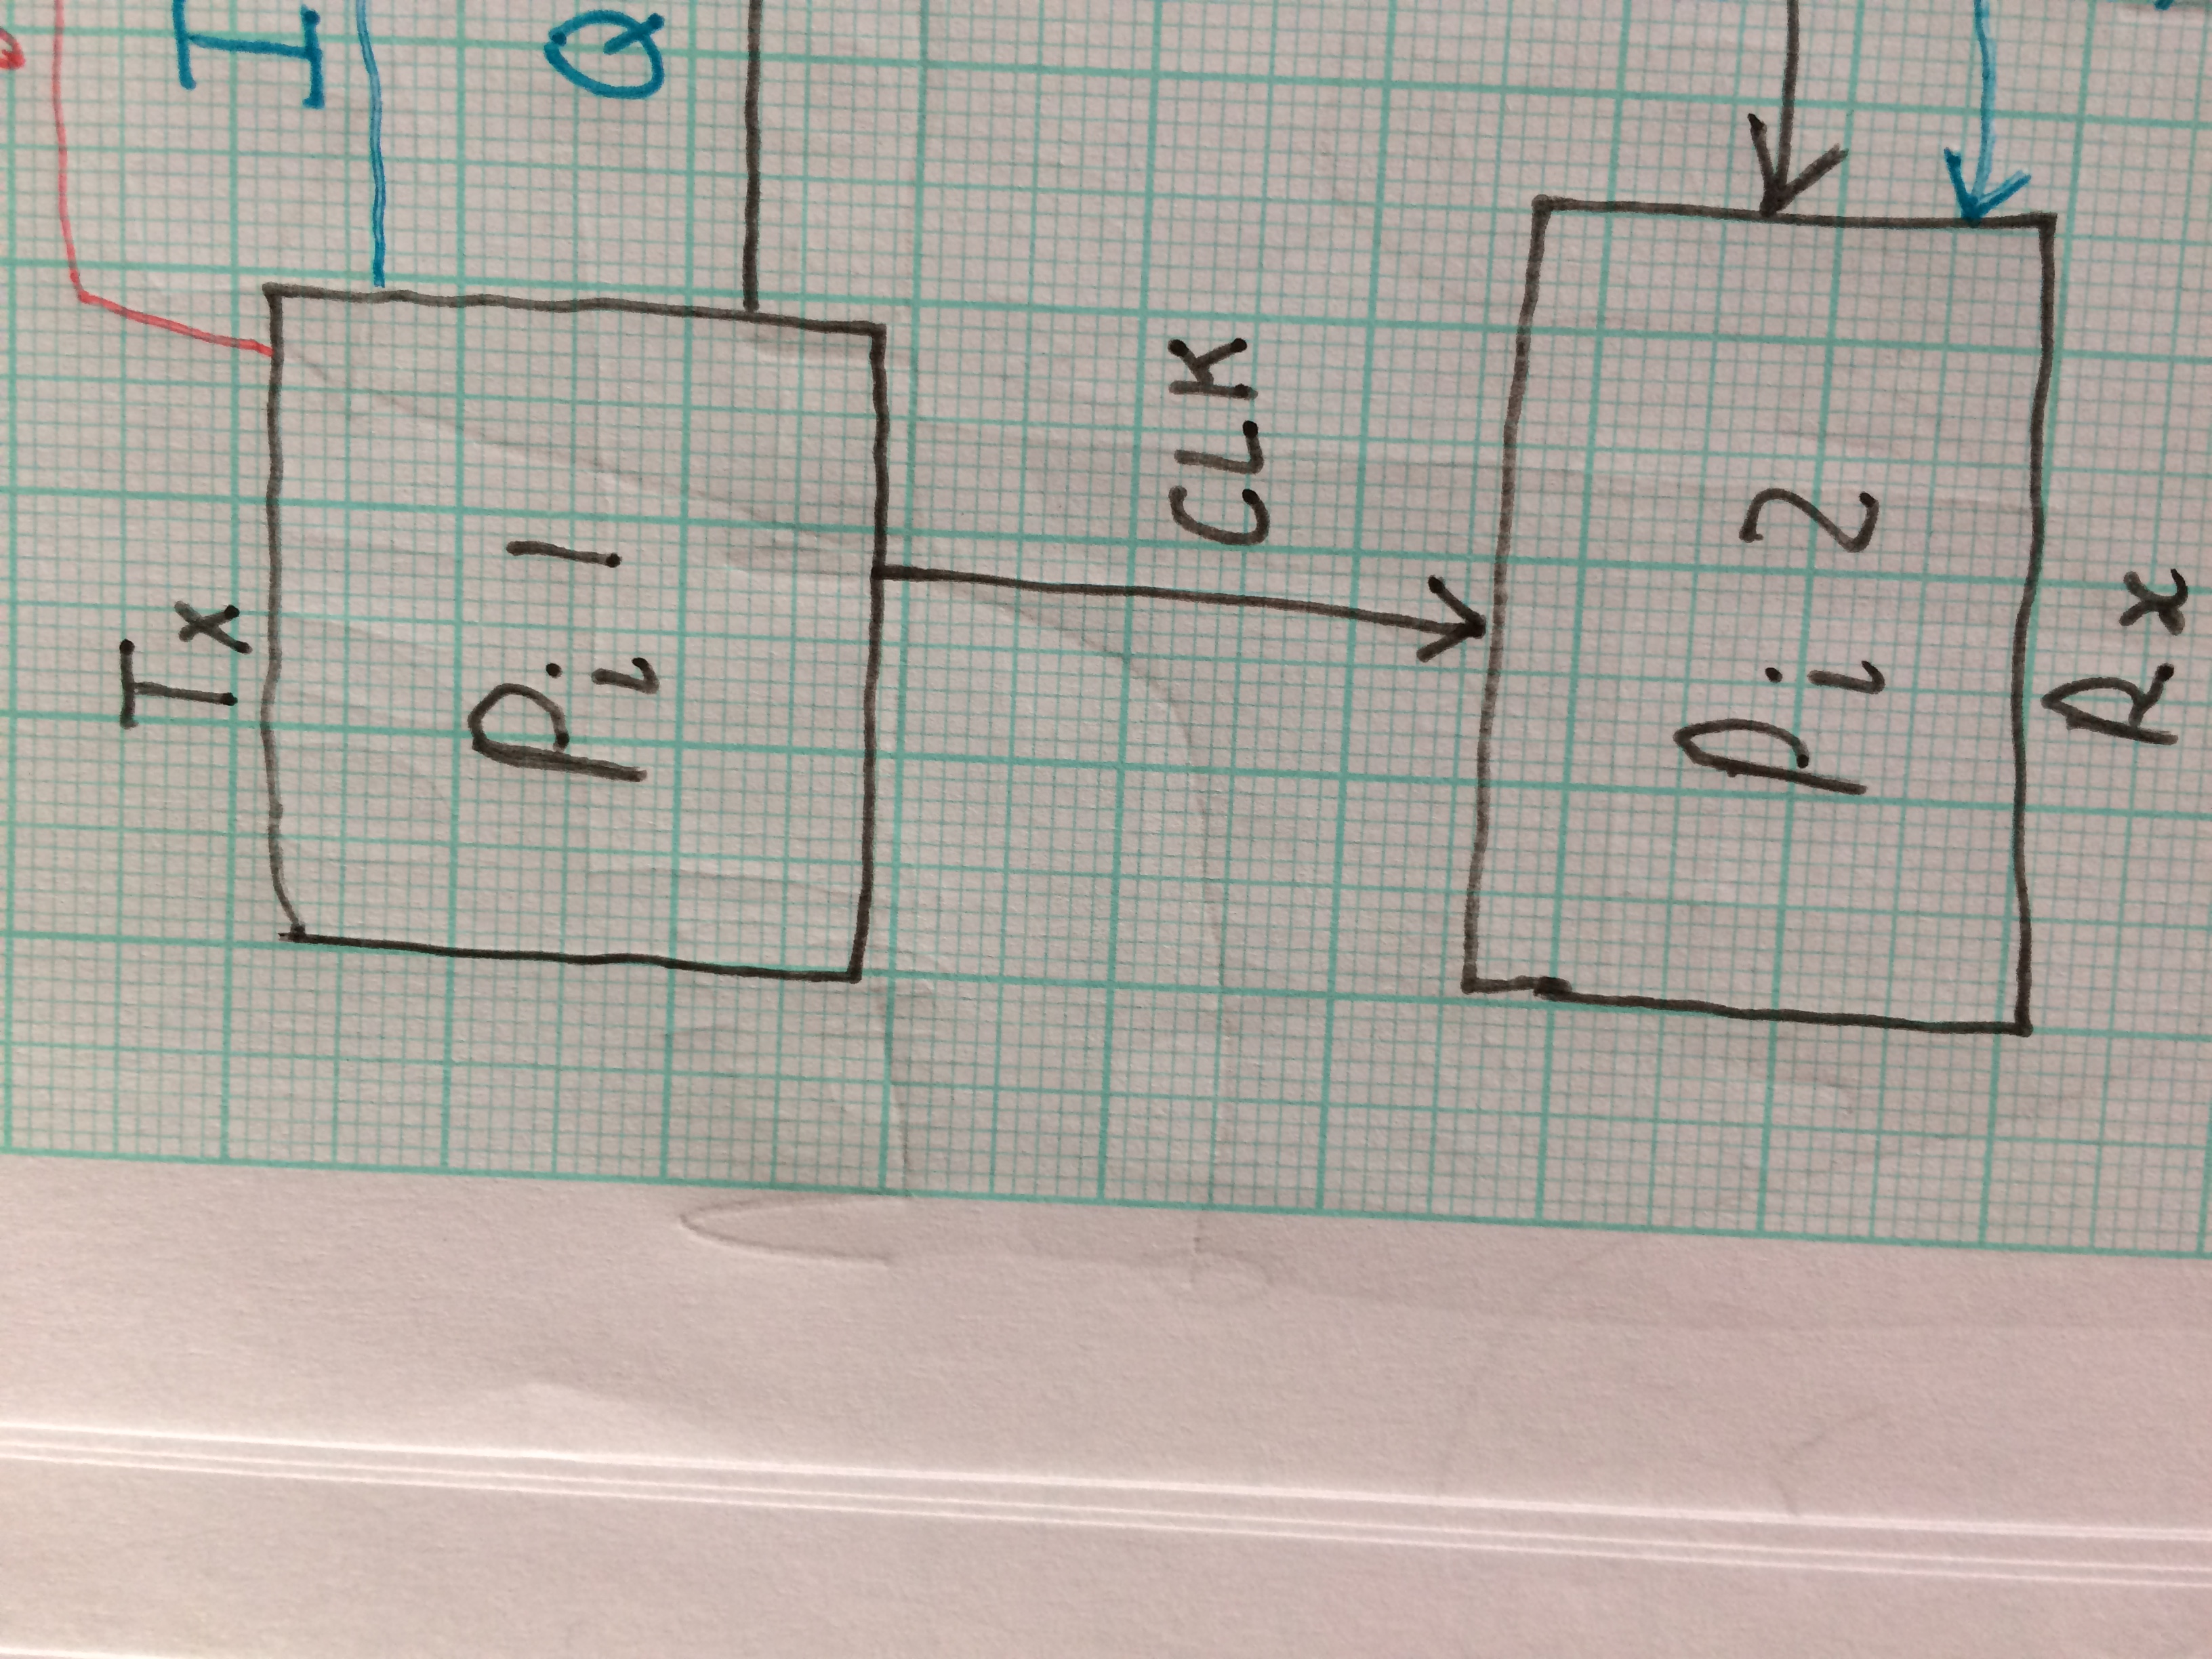
\includegraphics[width=0.6\textwidth]{OOK_Architecture.jpg}
	\caption{Test Bed Set-up For On-Off Keying}
	\label{fig_OOK Architecture}
\end{figure}

\subsection{Digital Analogue Converter}

The Digital Analogue Converter used is the AD5424, an 8-bit CMOS current output DAC with an easy interface to microcontrollers.
It has a \SI{17}{\nano\second} write cycle and a maximum update rate of \SI{20.4}{MSPS}. % Mega Samples Per Second
The converter is set up with a non-inverting operational amplifier to produce a full-range voltage output.
The Read/Write ($R/\overline{W}$) pin is pulled low permanently so the chip is in write mode; read back of the parallel digital outputs is not required.
The Chip Select pin ($\overline{CS}$) needs a falling edge and a rising edge to complete a write cycle, where the rising edge loads new parallel data, so this is connected to the clock pin of the Raspberry Pi.
Layout of the connections to the Pi are in the Figure \ref{fig_DAC Layout}.\\

\begin{figure}[ht]
	\centering
	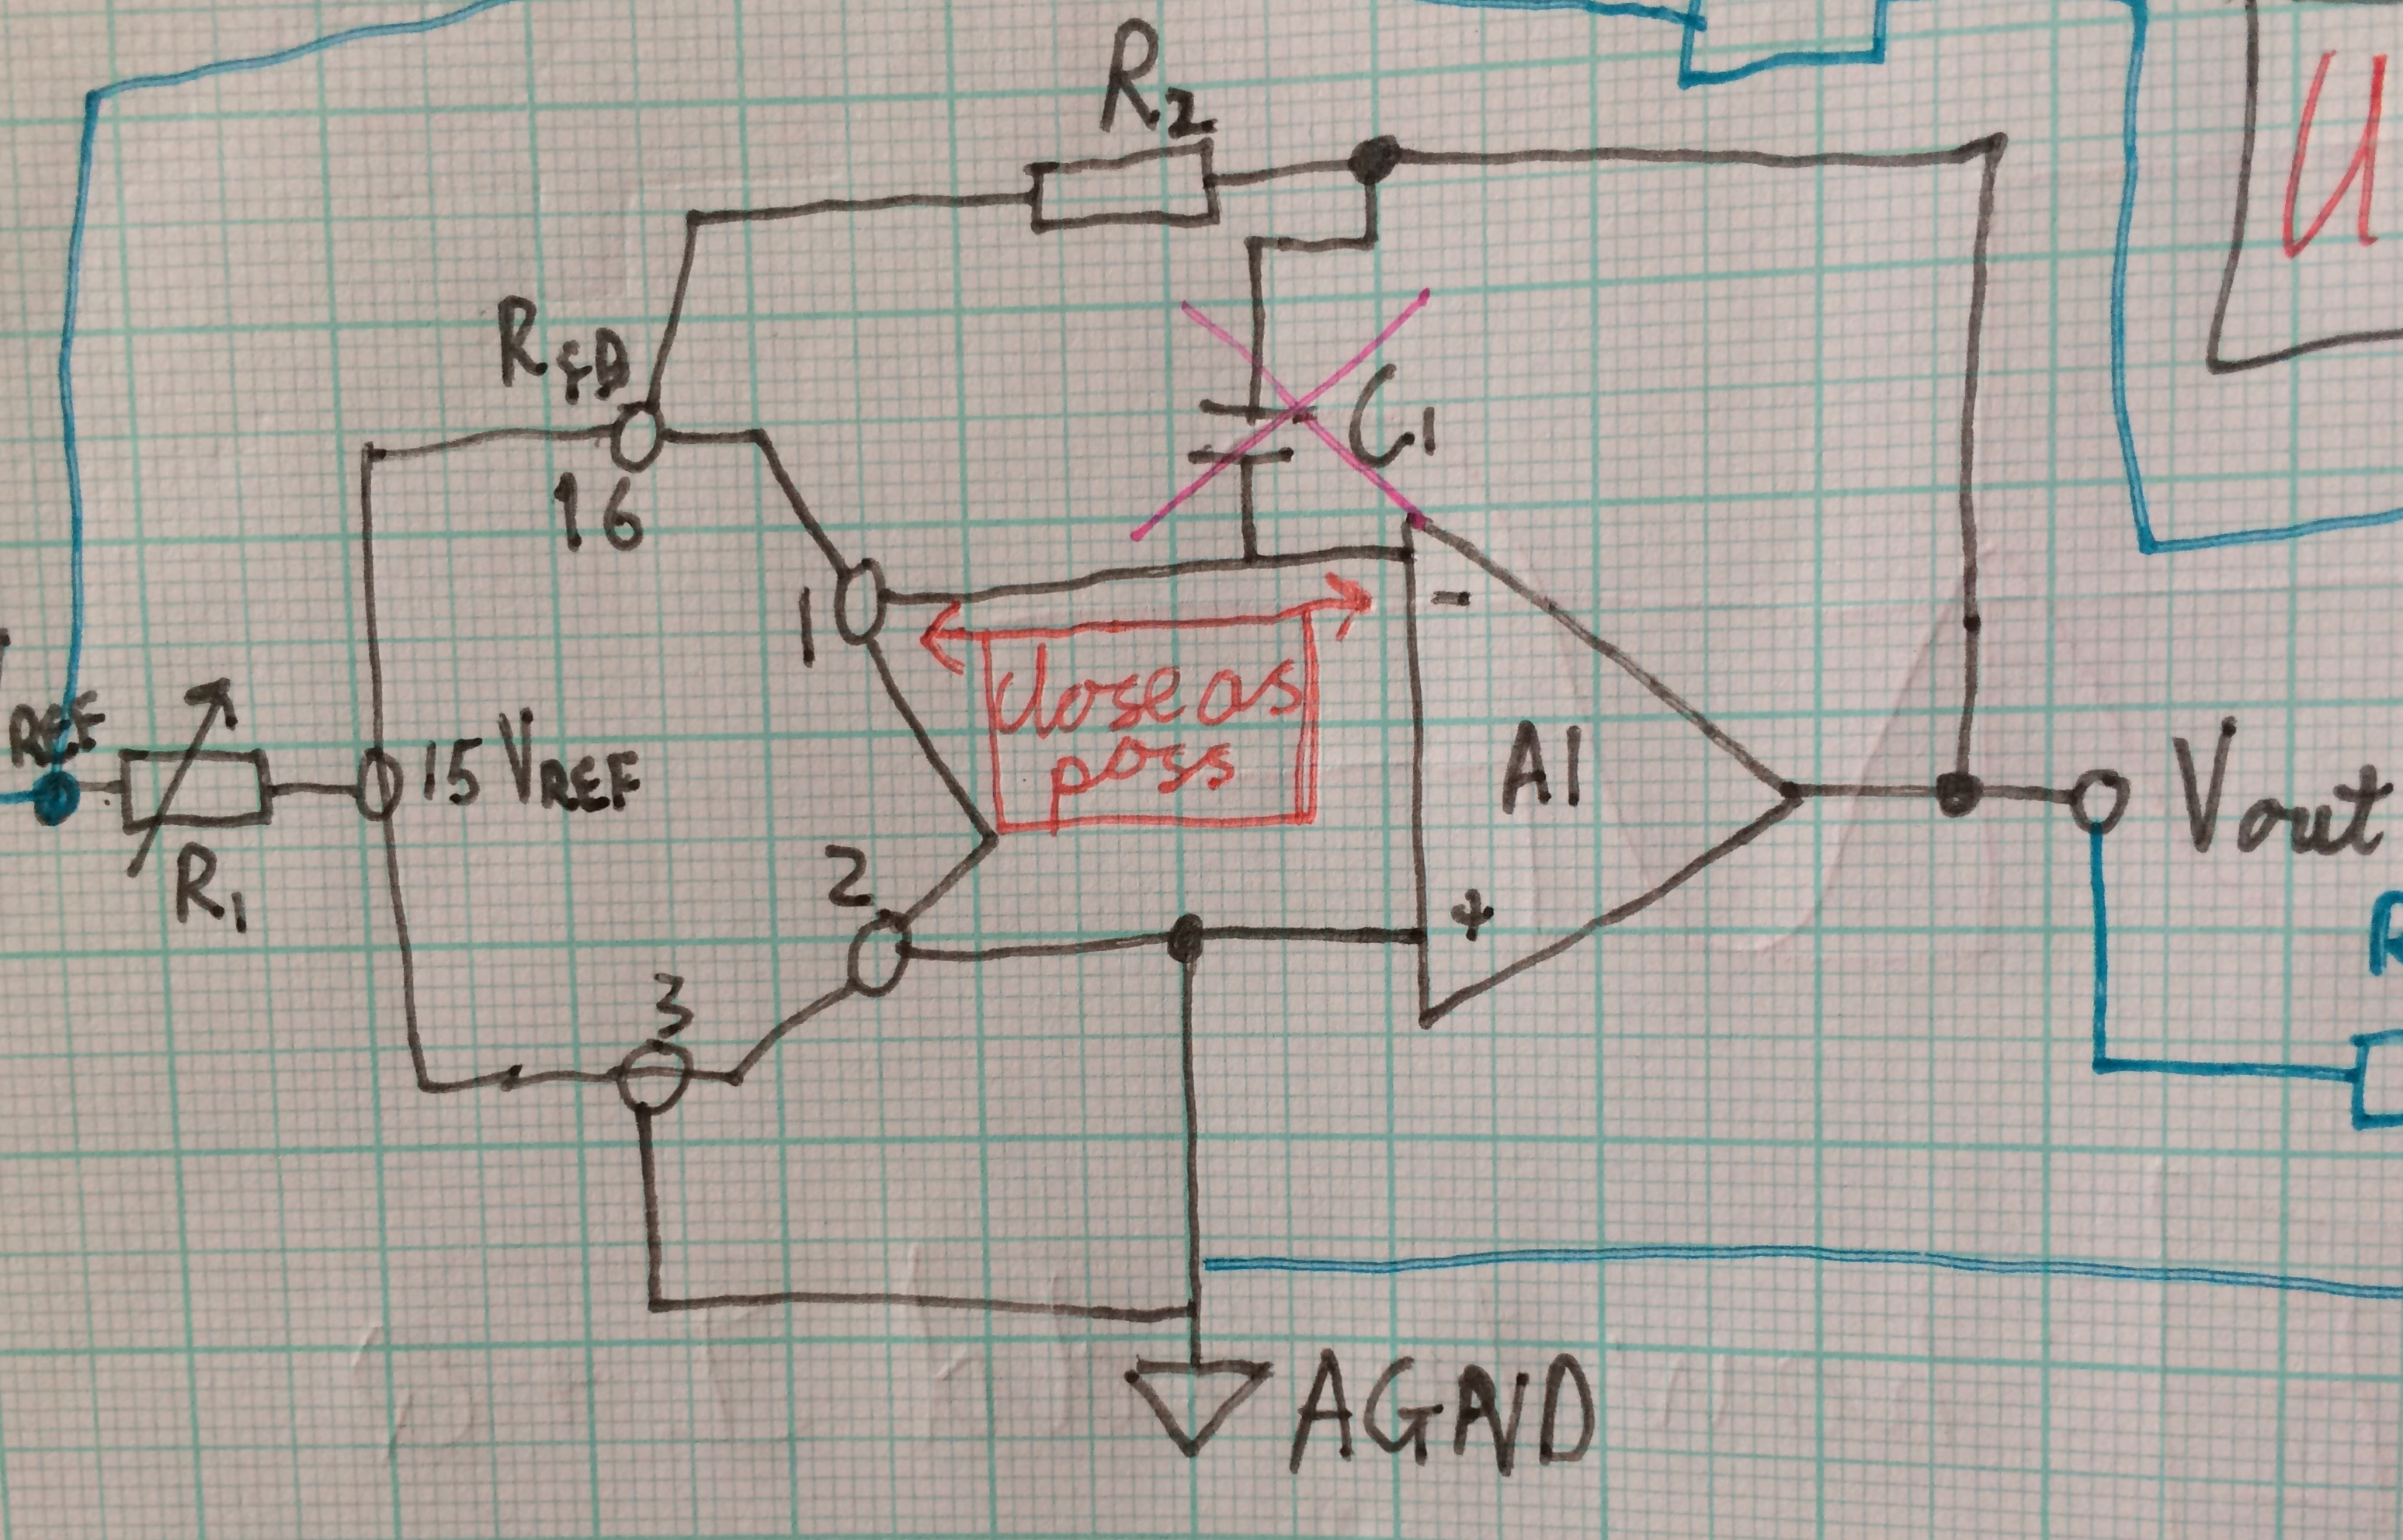
\includegraphics[width=0.6\textwidth]{DAC_Layout.jpg}
	\caption{Layout of the Digital Analogue Converter}
	\label{fig_DAC Layout}
\end{figure}

\subsection{Analogue Digital Converter}

The Analogue Digital Converter used is the ZN448, 

\missingfigure{Layout of Digital Analogue Converter}

\begin{figure}[ht]
	\centering
	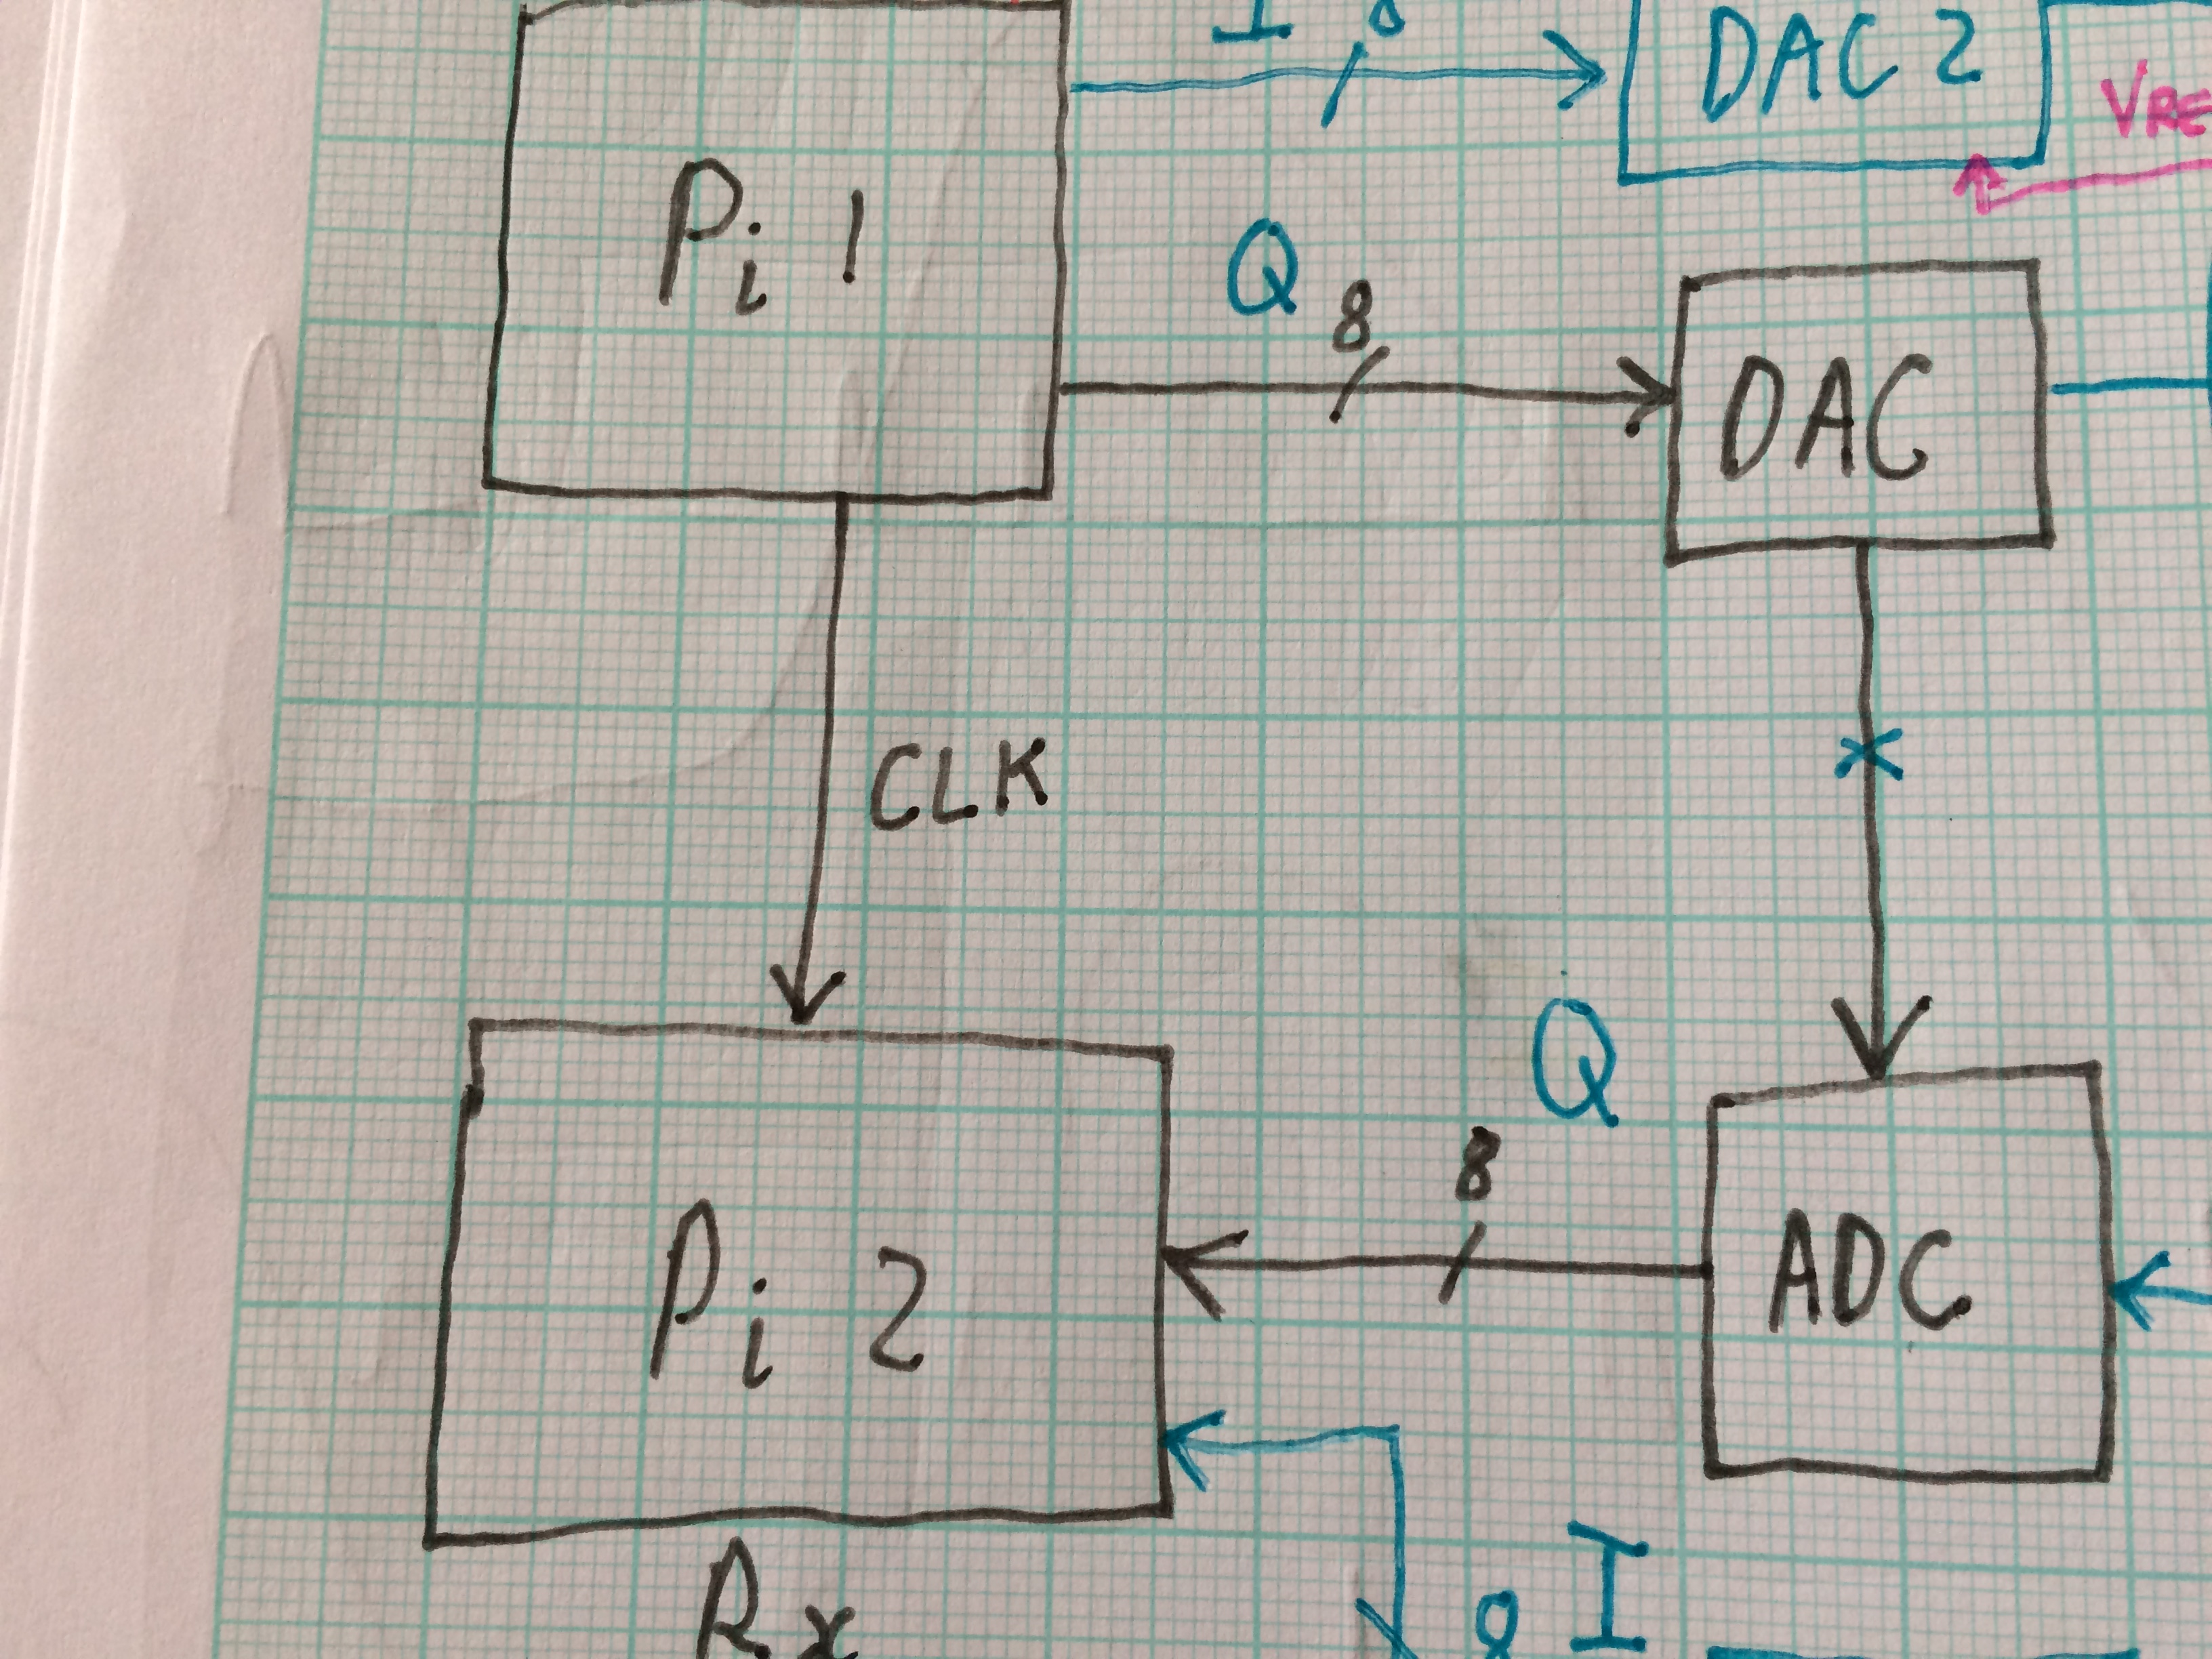
\includegraphics[width=0.6\textwidth]{PAM_Architecture.jpg}
	\caption{Layout for Pulse Amplitude Modulation}
	%\label{fig_}
\end{figure}

\subsection{Multiplier} \label{sec_Multiplier}

\todo[inline]{Depending whether it's doable, include  this section without multipliers on transmitter, pseudo ground on output}

\begin{figure}[ht]
	\centering
	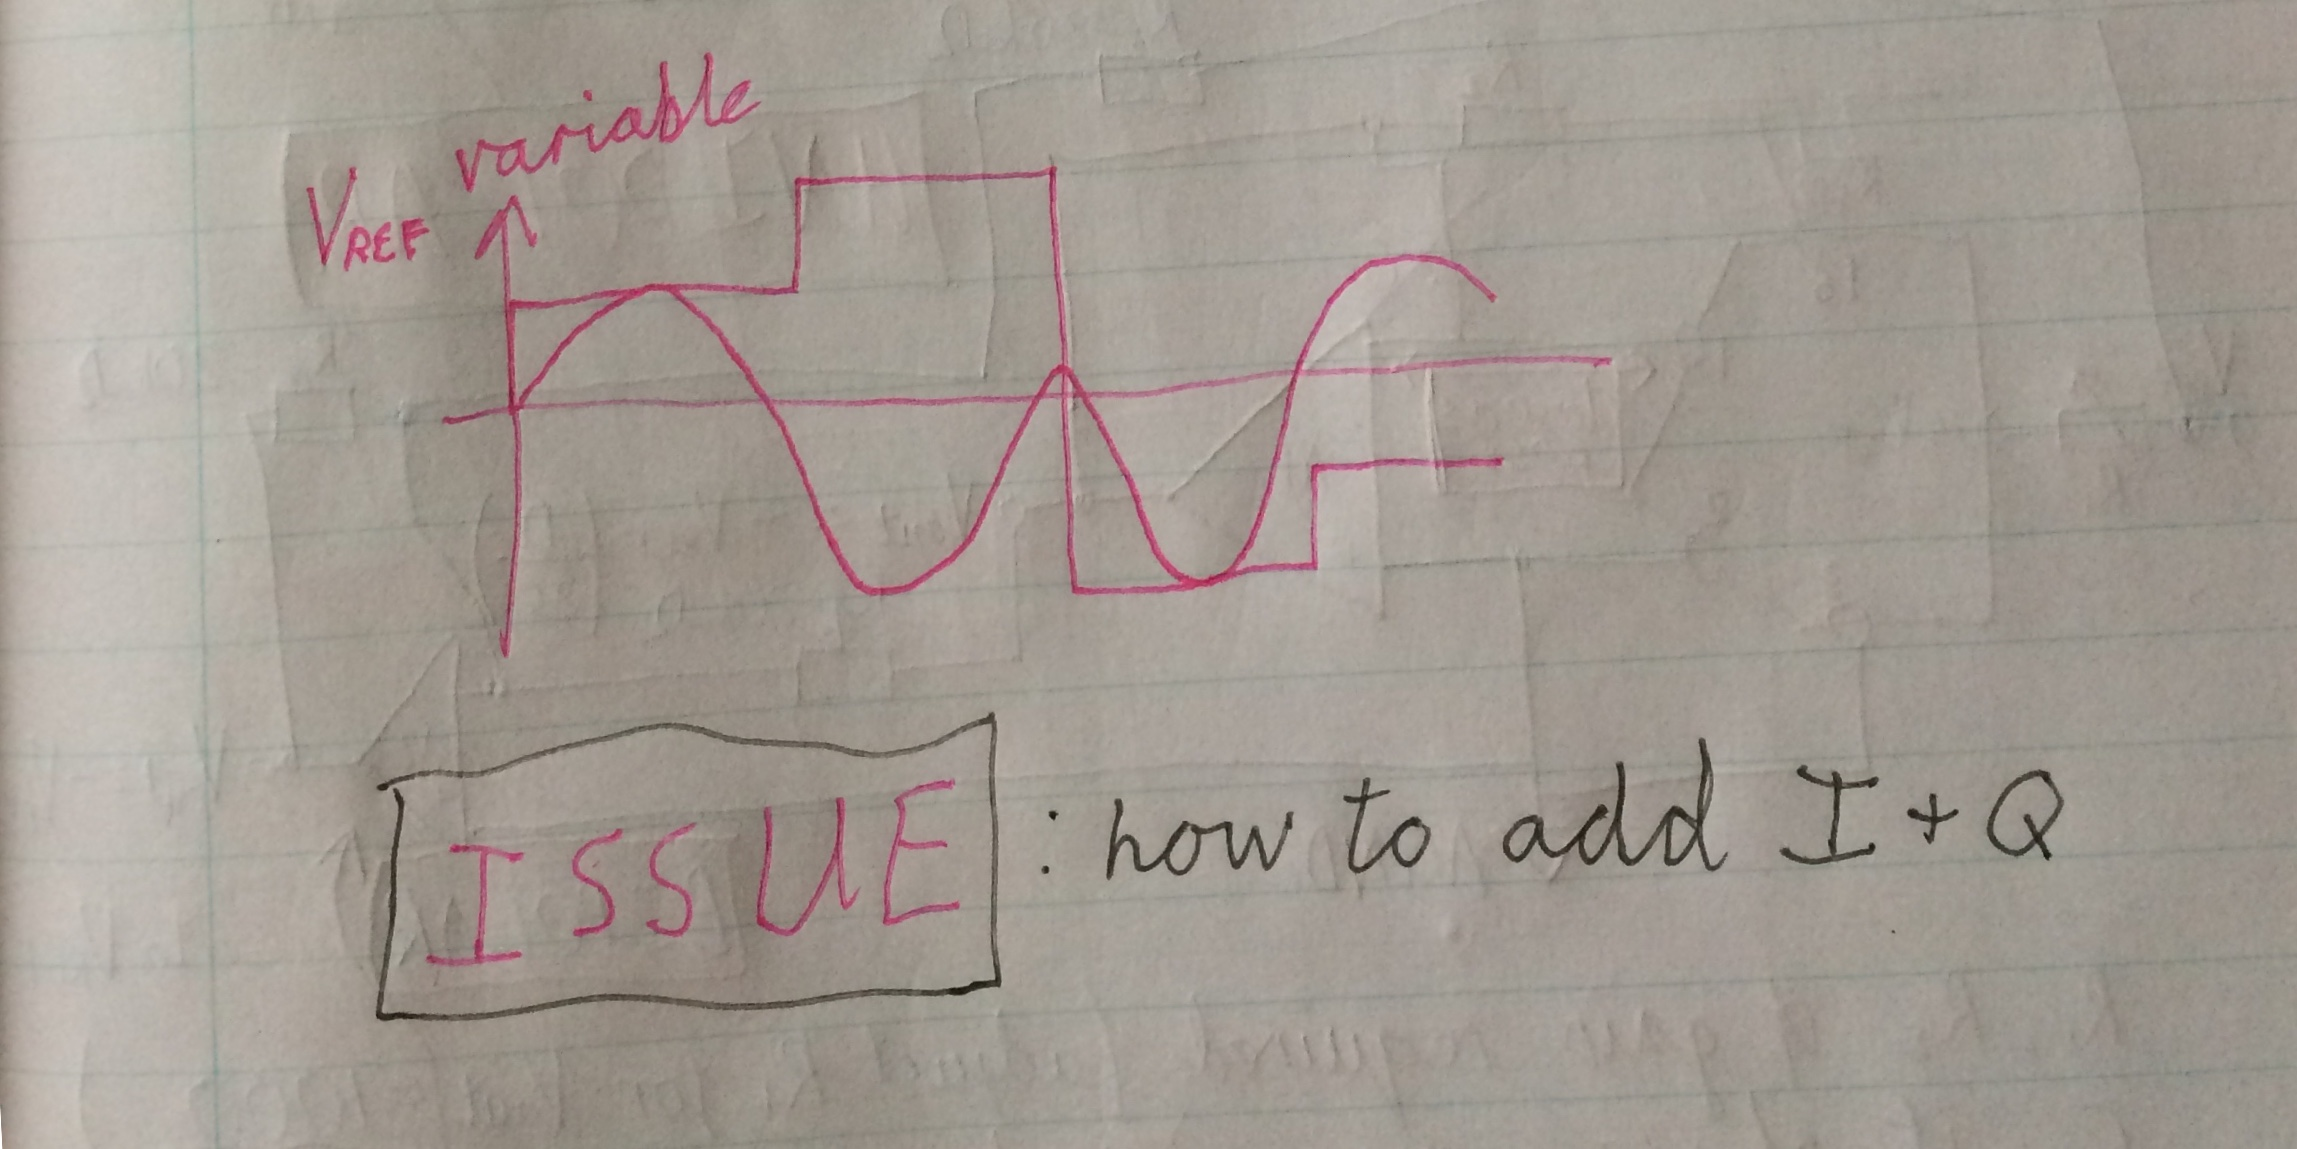
\includegraphics[width=0.6\textwidth]{DAC_Modulation.jpg}
	\caption{Four Quadrant Multiplication of input sinusoid using DAC}
	%\label{fig_}
\end{figure}

The Pi is not able to output negative voltages. Thus, Pulse Amplitude Modulation
uses the range 0 to Vmax not -Vmax to Vmax. Similarly, QAM uses a grid all in
the positive quadrant (0,1,2,3 not -3,-1,1,3). The same "negative" effect is still
achieved by using the "GROUND" of the multipliers (which are fully differential)
as Vmax/2 using a voltage divider. This means the sine and cos will be inverted
for the values 0 and 1 in the same way they would be for -3 and -1 and the
transmitted signal

\begin{figure}[ht]
	\centering
	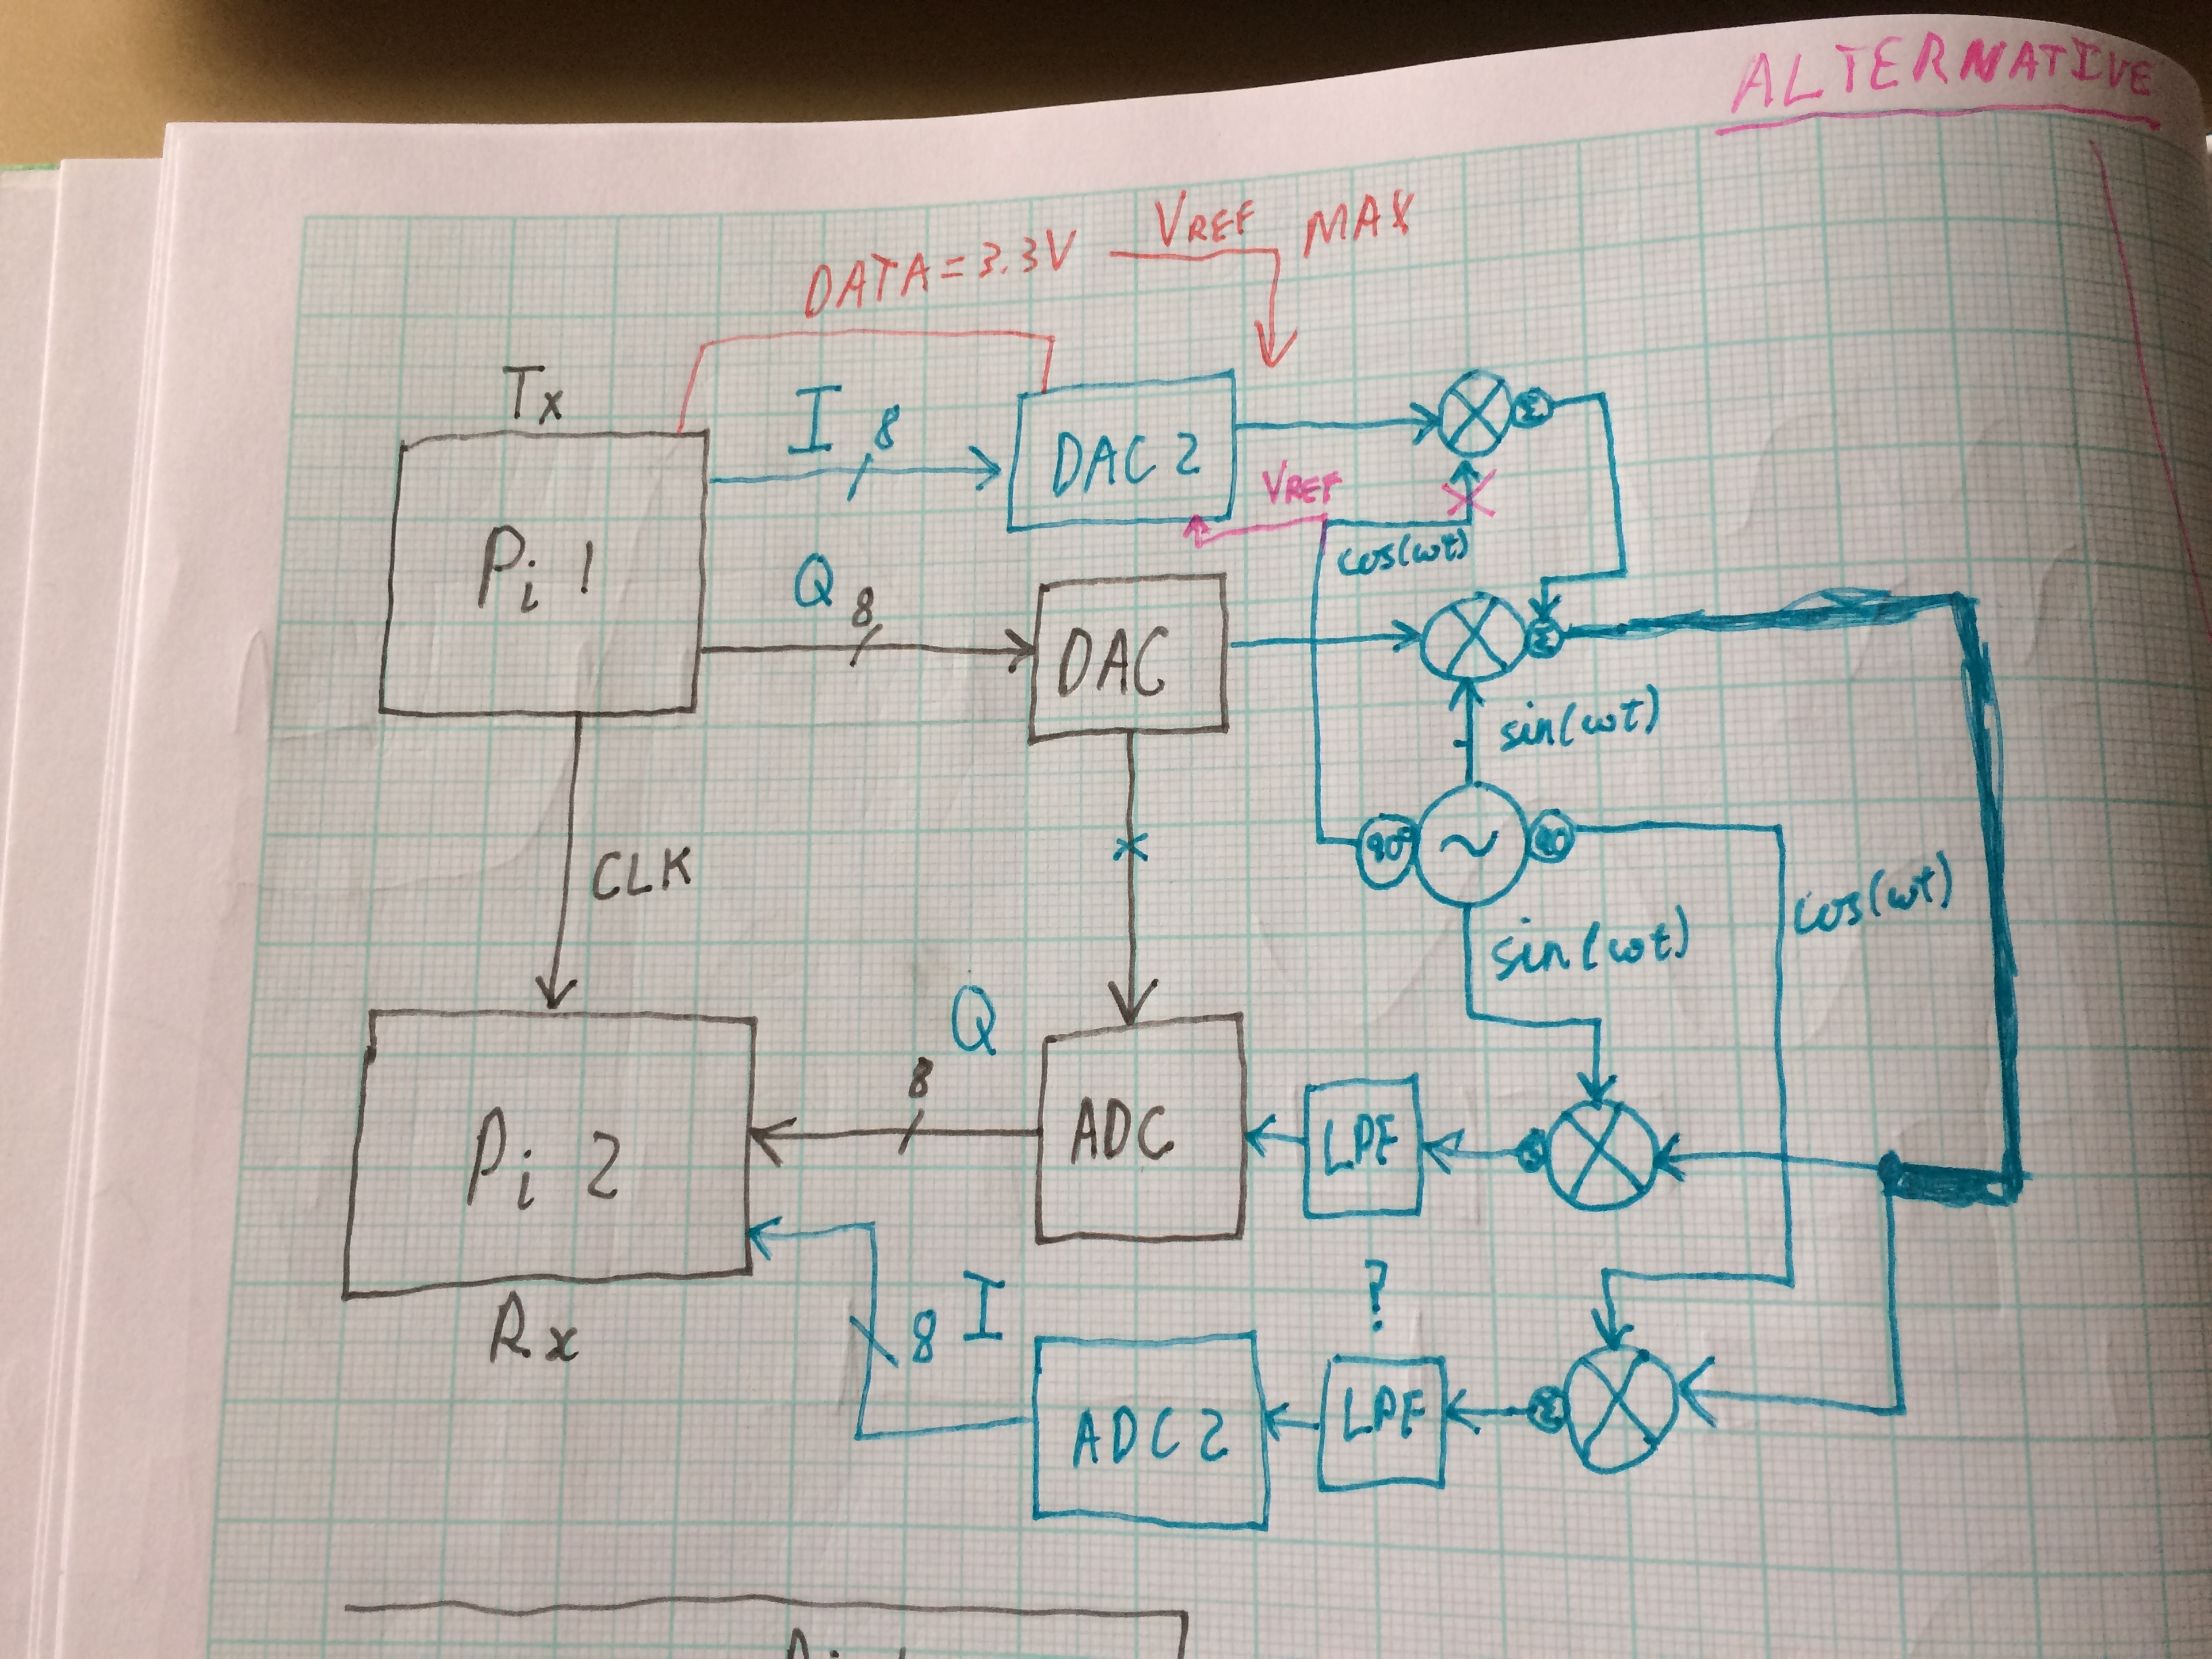
\includegraphics[width=0.6\textwidth]{QAM_OFDM_Architecture.jpg}
	\caption{Layout for Quadrature Amplitude Modulation and Potentially Orthogonal Frequency Division Multiplexing}
	%\label{fig_}
\end{figure}

\subsection{Parts Used}

\todo[inline,color=green!40]{Need a diagramatic representation as well as an actual picture}
\begin{figure}[ht]
	\centering
	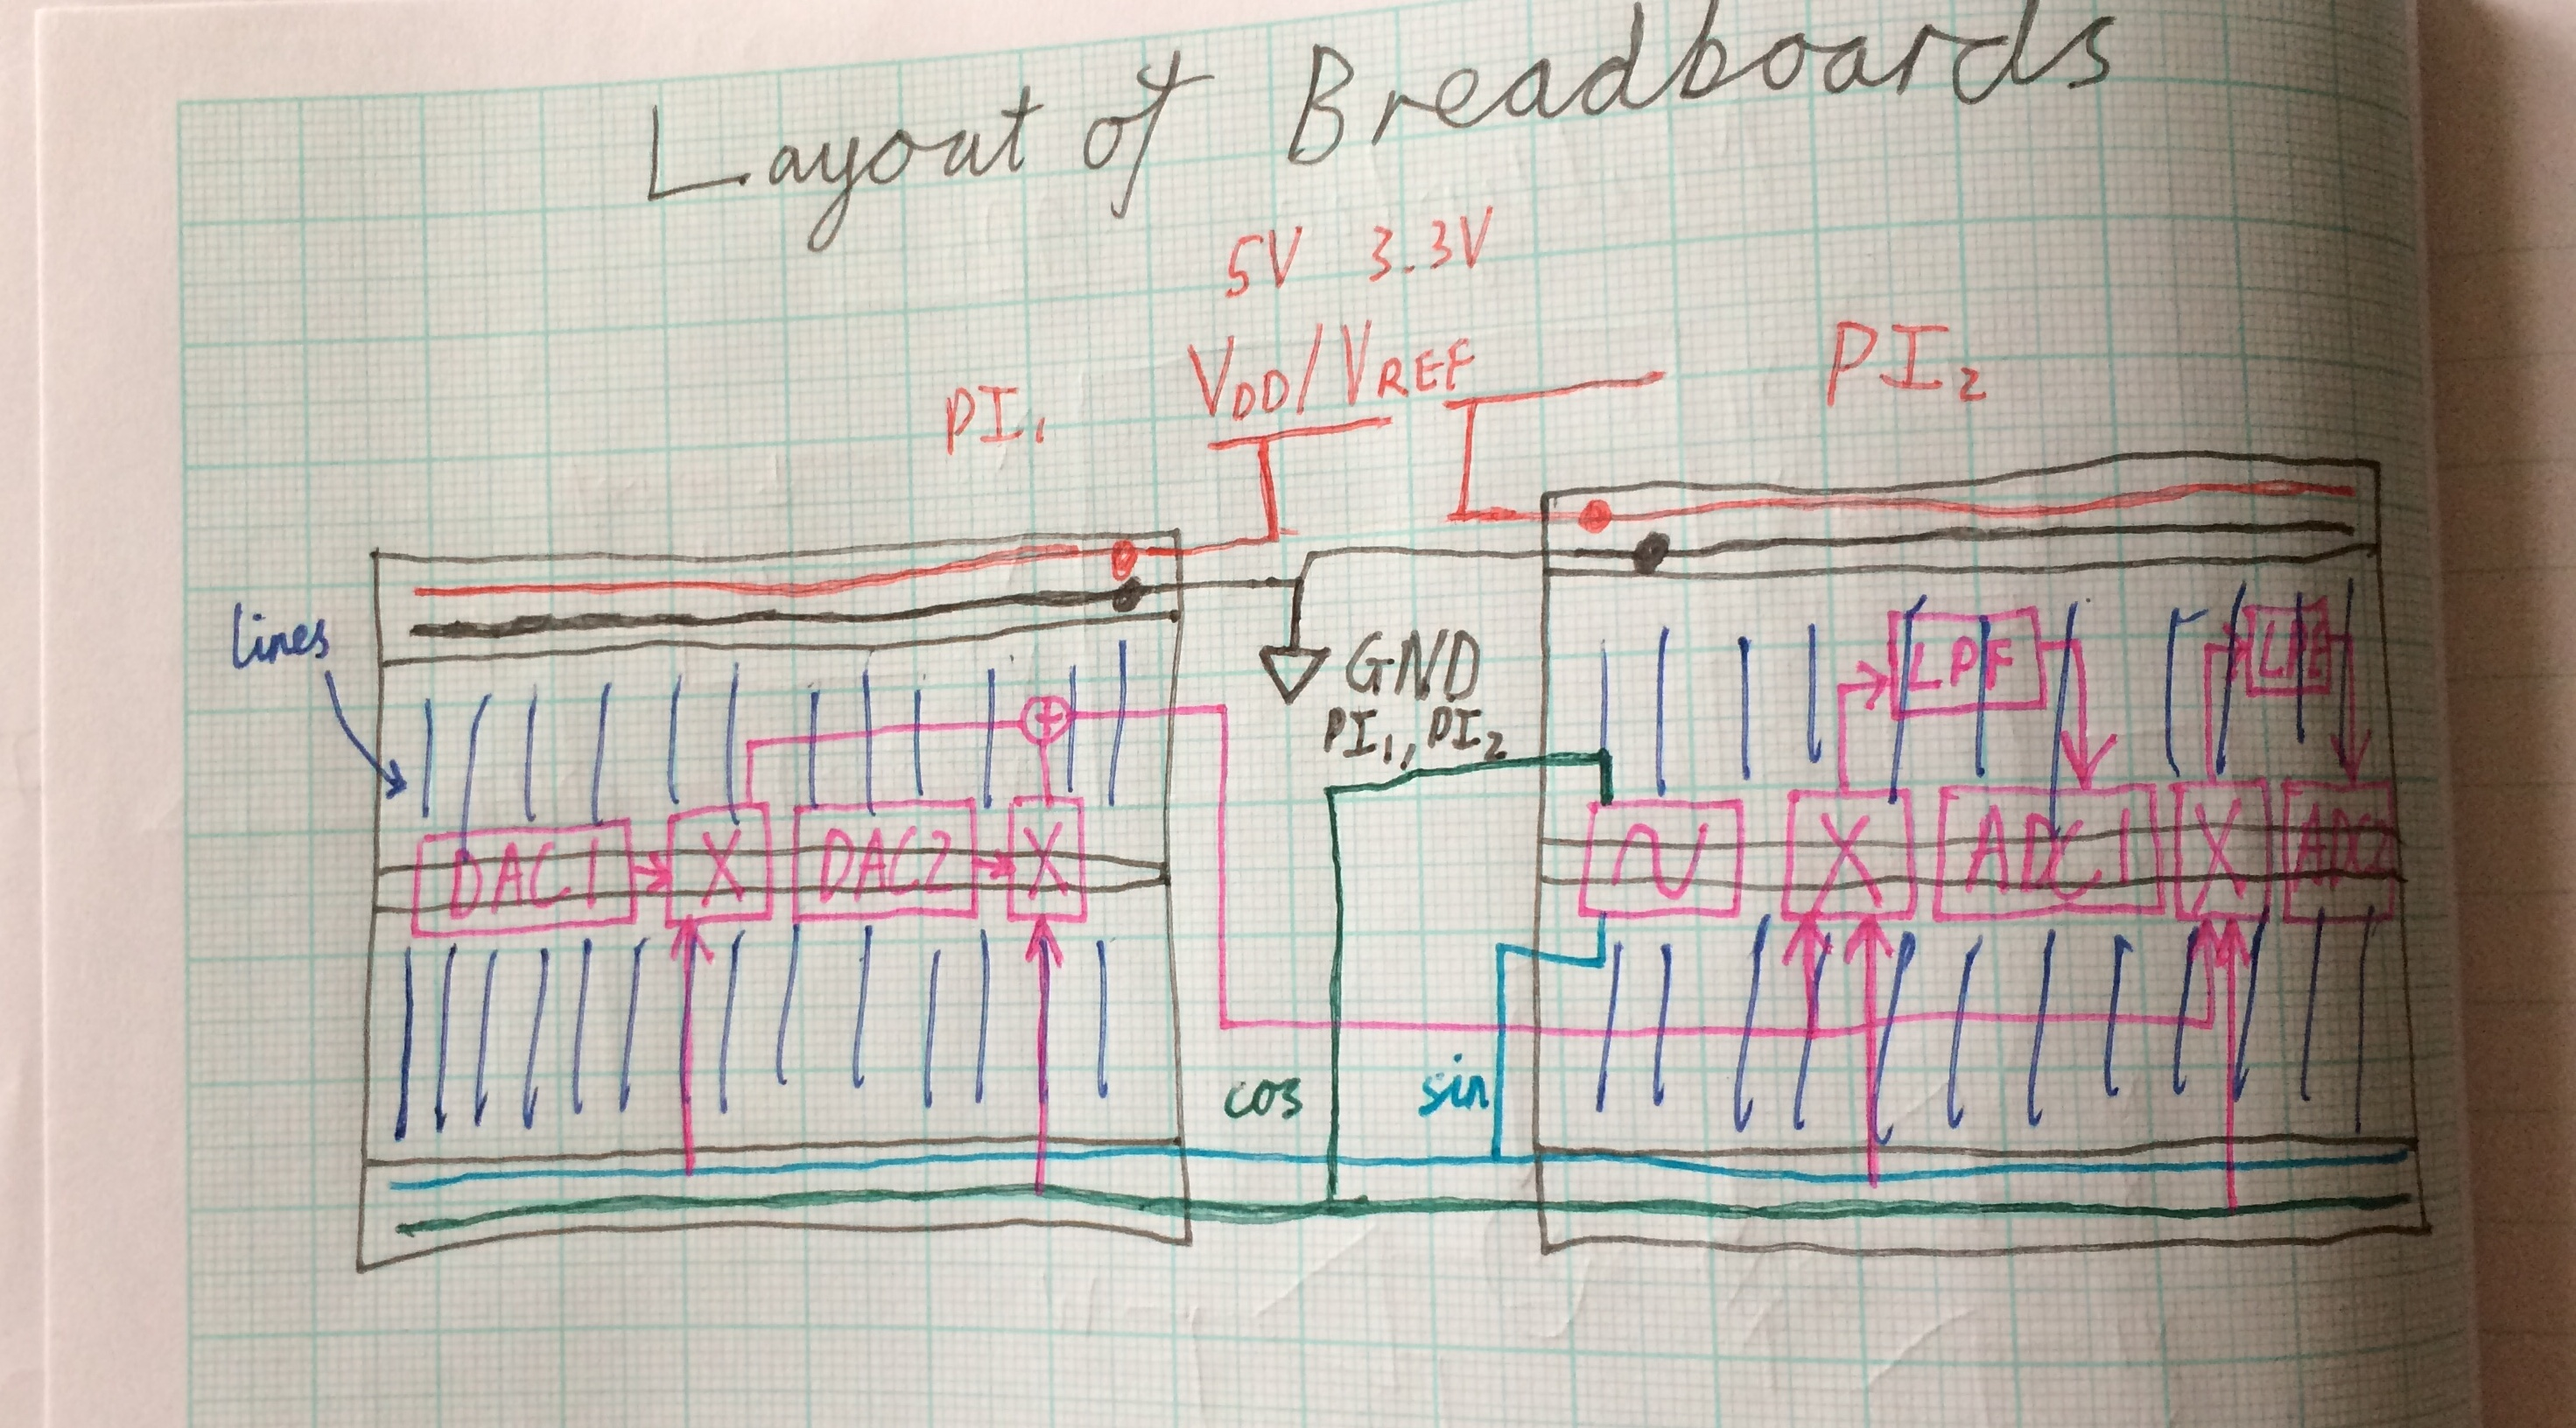
\includegraphics[width=0.6\textwidth]{Live_Test_Bed.jpg}
	\caption{What the Test Bed Actually Looks Like in its Final Configuration}
	%\label{fig_}
\end{figure}

\todo[inline,color=blue!20]{Include a section on pricing of the parts and comparison to actually used test beds}

It is worth noting that there is a large variety of available options for each component of the test bed.
Each possibility has certain advantages and disadvantages, and a lot of the options are not suitable due to the power requirements or ease of interfacing with the Raspberry Pi.
As a result of this, the parts used in this project were the most suitable parts which could be found and successfully sourced.
However, there may be more suitable chips available given more time or experience, and being aware of this would be useful if this project were to be extended and/or replicated.
All parts could be replaced with minimal adjustment to the set-up and code.\\

Changes which would be made with hindsight, if components with the required qualities could be found, are as follows:

\todo[inline,color=blue!20]{Continue to add to this list as you write the Architecture section - remove redundant information already discussed in earlier sections}
\begin{itemize}
	\item A number of chips used are surface mounted, requiring difficult soldering to solder pads, This would be useful if they were to be used on a printed circuit board for a final design, but on a prototyping breadboard, dual in-line packages would have been easier to use where available
	\item The Digital Analogue Converter was chosen for its easy interfacing with a microcontroller, but a voltage-output device would remove the need to use additional operational amplifiers at the output. It also had some issues with correct values and it is unclear if it was the implementation or the chip itself.
	\item Analogue Digital Converter
	\item The Quadrature Sinusoid Generator uses an oscillator chip which outputs $90^o$ out-of-phase square waves, and the used chip was the only simple one which did this. Ideally the outputs would already be sinusoidal (one quadrature chip or a sine generator and phase shifter) so that low pass filters with fixed frequency response could be omitted to make changing the carrier frequency purely software-dependent.
	\todo[inline]{Make sure I am consistent with use of Quadrature Sinusoid Generator vs Oscillator in report}	
	\item The multiplier is designed to operate around \SI{10}{\volt}, and so has a built in \SI{10}{\volt} normalisation in the multiple which attenuates the signal and required re-amplification before transmission. A similar chip designed for lower voltages would be ideal.
	\todo[inline]{Fact check this}
	\item Low Pass Filters
\end{itemize}

\clearpage

%%%%%%%%%%%%%%%%%%%%%%%%%%%%%%%%%%%%%%%%%%%%%%%%%%%%%%%%%%%%%%%%%%%%%%%%%%%%%%%%%%%%%%%%%%%%%%%%%%%%%%%%%%%%%%%%%%%%%%%%%%%%%%%%%%

\section{Programming}

The Raspberry Pi is used for its low cost, ease of use, and the fact that it has programmable Input/Output (I/O) pins.
The I/O pins can be programmed using different libraries in Python and C.
The standard GPIO library which comes installed with Raspbian is RPi.GPIO for Python \ref{web_RPi.GPIO}.
\todo[inline,color=green!40]{Add bib reference to RPi.GPIO https://pypi.python.org/pypi/RPi.GPIO}
This is used for the On-Off Keying part of the communications test bed.
The Python library is slow however, and so a C library is used for the pin-level manipulation for all modulation schemes requiring multi-level outputs through Digital Analogue Converters.
This is done both for the improved speed performance of the C library, and the capability of this library to output to multiple pins at once.
Section \ref{sec_Comparing Python and C} goes into a detailed  investigation of the differences between these options.
\todo[inline]{CHECK - Do I need to change this from my name to an anonymous account if only candidate number is on cover page}
All of the code and the report for the project are maintained on GitHub, and may be found at \url{https://github.com/CamEadie/4YP_PiCom}.\\

The transmitter and receiver code for all modulation schemes considered works from a single final version of the test bed.
This consists of the Python transmitter \textit{PiComTx\textunderscore 5\textunderscore DAC.py} and receiver \textit{PiComRx\textunderscore 5\textunderscore DAC.py} files, and the executables compiled from C code for the transmitter \textit{PiTransmit\textunderscore 3} and receiver \textit{PiReceive}.
The body of the main Python codes for each the transmitter and receiver is split into OOK and Advanced Modulation Schemes.
On-Off Keying (Section \ref{sec_On-Off Keying}) is the simplest form of clocked communication possible, and acts as a proof of concept for the Raspberry Pis as a test bed.
It is implemented using a native Python list which stores '1's and '0's to represent the binary stream, and these are output using the native RPi.GPIO library.
The OOK was added into the final code of the Advanced Modulation Schemes (Section \ref{sec_Advanced Modulation Schemes})  from previous versions retrospectively, as all of the Advances Schemes are implemented in the same code.
This was done both to make it easier to conduct all tests through one program, and to adhere to the idea of Software Defined Radio being as change-independent as possible (Section \ref{sec_Lit Review}).\\
\todo[inline,color=green!40]{Rephrase this and make sure the section referenced is as consistent with this comment as possible}
The Advanced Schemes considered are 4-level Pulse Amplitude Modulation, 256-level Pulse Amplitude Modulation (used more for setting up the DAC and ADC, as differentiating between levels this precisely is not viable), 16-Quadrature Amplitude Modulation and Orthogonal Frequency Division Multiplexing.
The code also improves the data manipulation, includes image handling so images can be transmitted allowing for visualisation of the error rate etc. of the transmission, and implements a separate compiled C module for the actual transmitting and receiving of data.\\

\begin{figure}[ht]
	\centering
	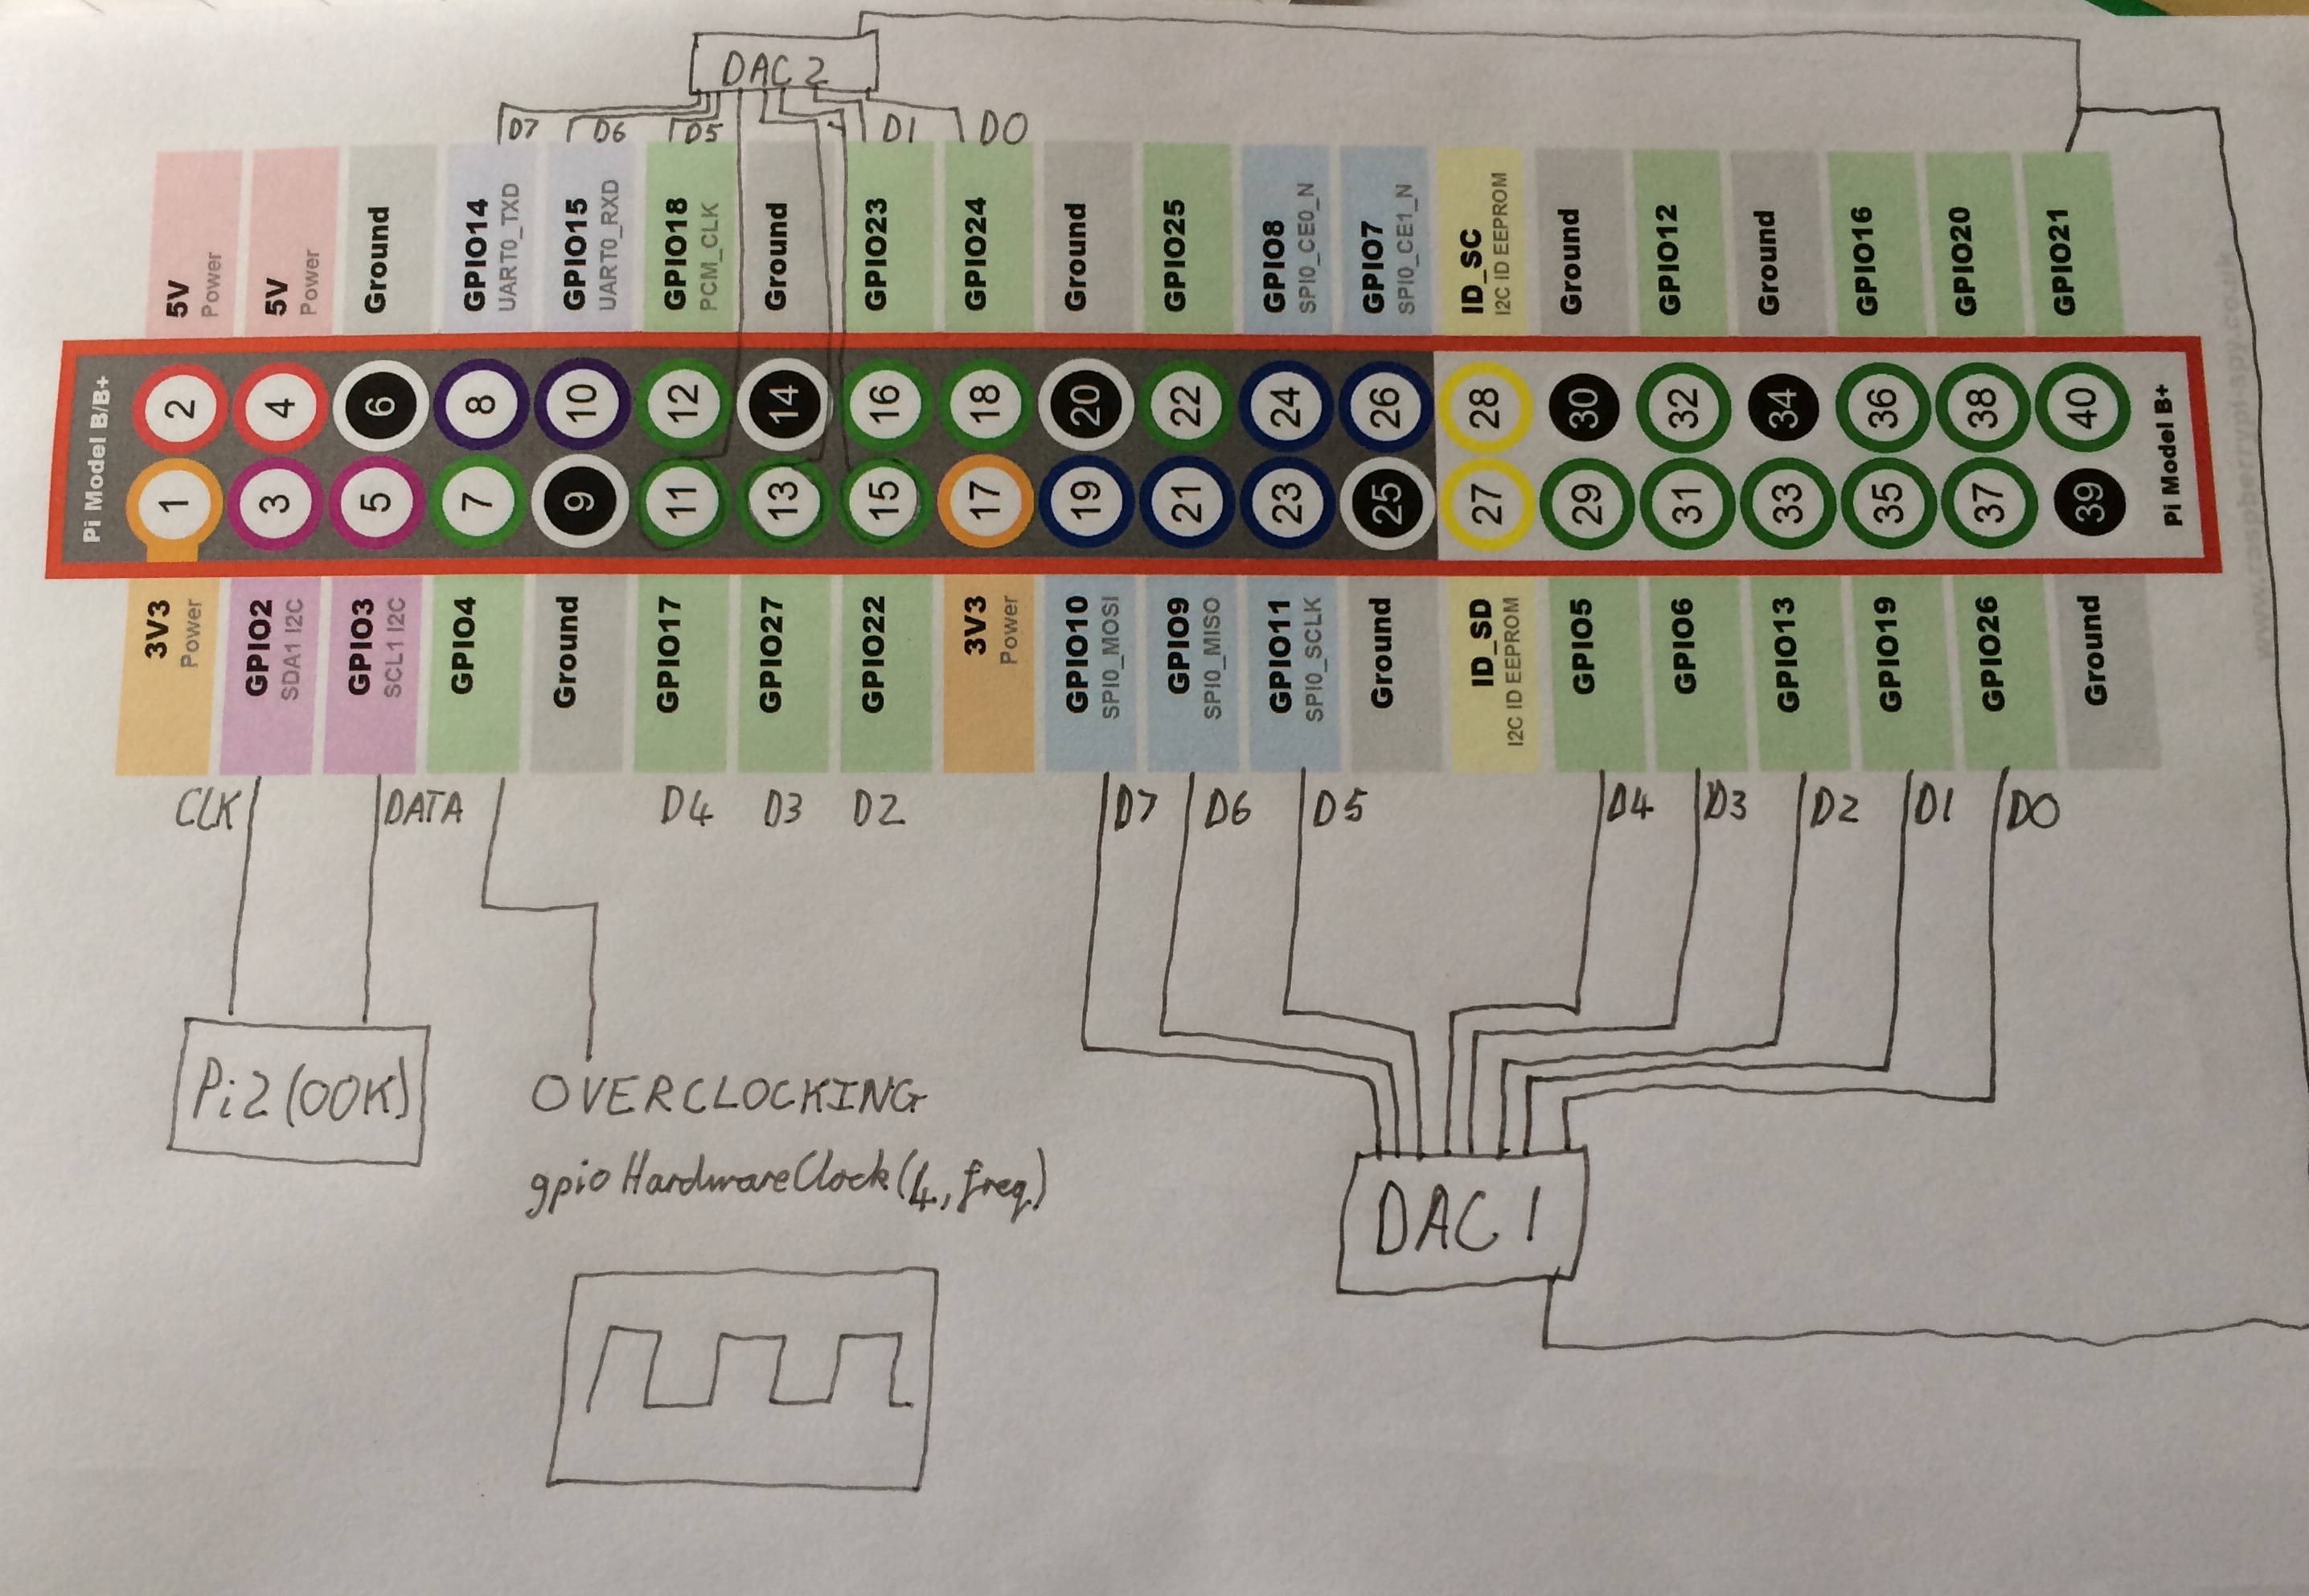
\includegraphics[width=0.6\textwidth]{Pi_Pin_Connections.jpg}
	\caption{Pin Diagram of Connections to Raspberry Pi (reference to image source) - These are alterable fairly easily in the code so changes can be made with little overhead}
	\label{fig_Pin Connections}
\end{figure}

\subsection{On-Off Keying} \label{sec_On-Off Keying}

On-Off Keying is a modulation scheme based on using $V_{max}$ as '1' and \SI{0}{\volt} as '0'.
The transmit section of the test bed loops through the data list, outputting each value followed by a clock pulse using the sleep function.
The speed and accuracy of the \textit{GPIO.output()} and \textit{sleep()} functions is covered in Section \ref{sec_Electro Testing}.
The receiver uses the function \textit{GPIO.wait\textunderscore for\textunderscore edge()} on rising edges of the clock pin to trigger reading of the data pin, and .\\

Earlier versions of this modulation scheme included a function \textit{Prep\textunderscore Binary\textunderscore Data()} which added initial and final padding to the data of '1's to prevent missing timing of the beginning and end of transmission.
The function also added a padding bit to the data when either value had been repeated a certain number of times (for example a '1' if '0' had been repeated 5 times in a row).
This function was removed when \textit{Encode\textunderscore Error\textunderscore Correction()} was included, as forward error correction was seen as a better way of avoiding these and other errors without including padding bits which could be difficult to remove if errors did occur in the code transmission.
The channel coding used is syndrome decoding and is discussed more in Section \ref{sec_Channel Coding}.\\


\subsubsection{Starting the Receiver}
\todo[inline]{Paramiko}

\subsection{Advanced Modulation Schemes} \label{sec_Advanced Modulation Schemes}

PAM - as mentioned in section \ref{sec_Multiplier} 0-3

256 PAM is similar to 4PAM and is not included for space and because it's not viable in this setup especially with the problem mentioned in Section \ref{sec_Components}.
\todo[inline,color=green!40]{Make sure the right section does reference the fact that the DAC doesn't work exactly as it's supposed to and how I dealt with it}
OFDM is also conceptualised here but due to the same problem, the continuous value issue mentioned above would need to be fixed before it could be implemented.

Here we will definitely talk about the transmitter generally.\\

\begin{figure}[ht]
	\centering
	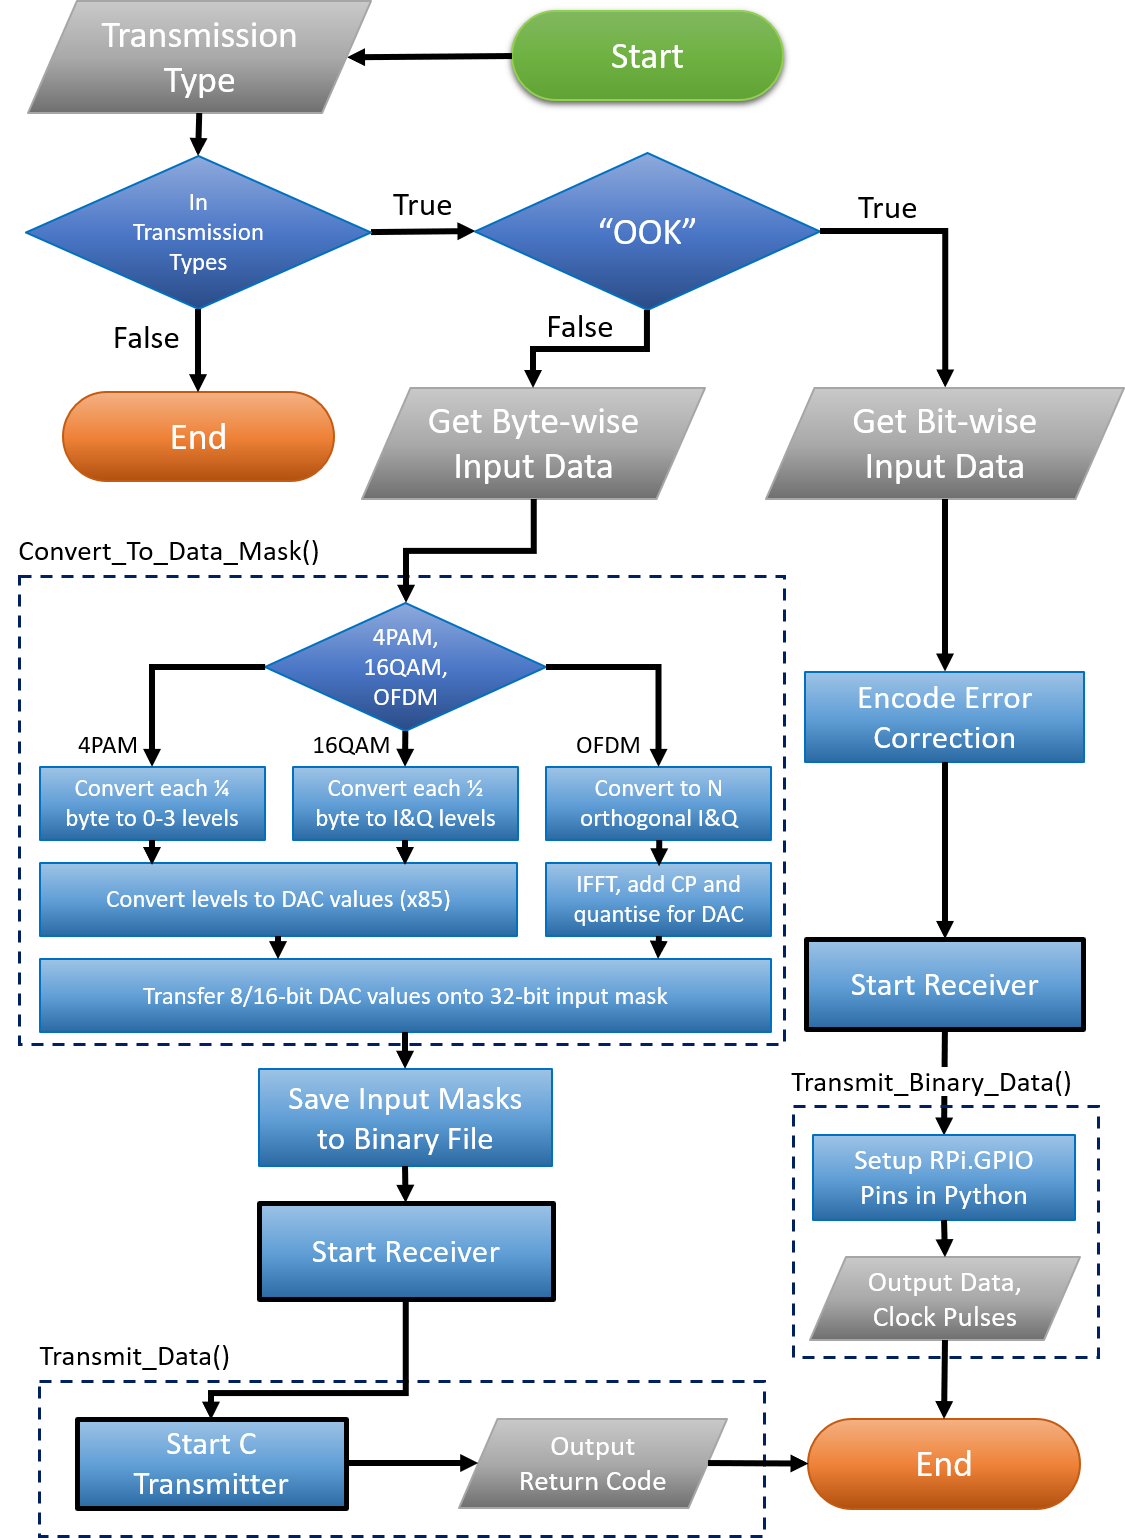
\includegraphics[width=\textwidth]{Transmitter_Flow.png}
	\caption{Flow Chart for Transmitter Code}
	\label{fig_Transmitter_Flow}
\end{figure}

Here we will definitely talk about the receiver generally enough to separate the flow charts by a page.\\

\begin{figure}[ht]
	\centering
	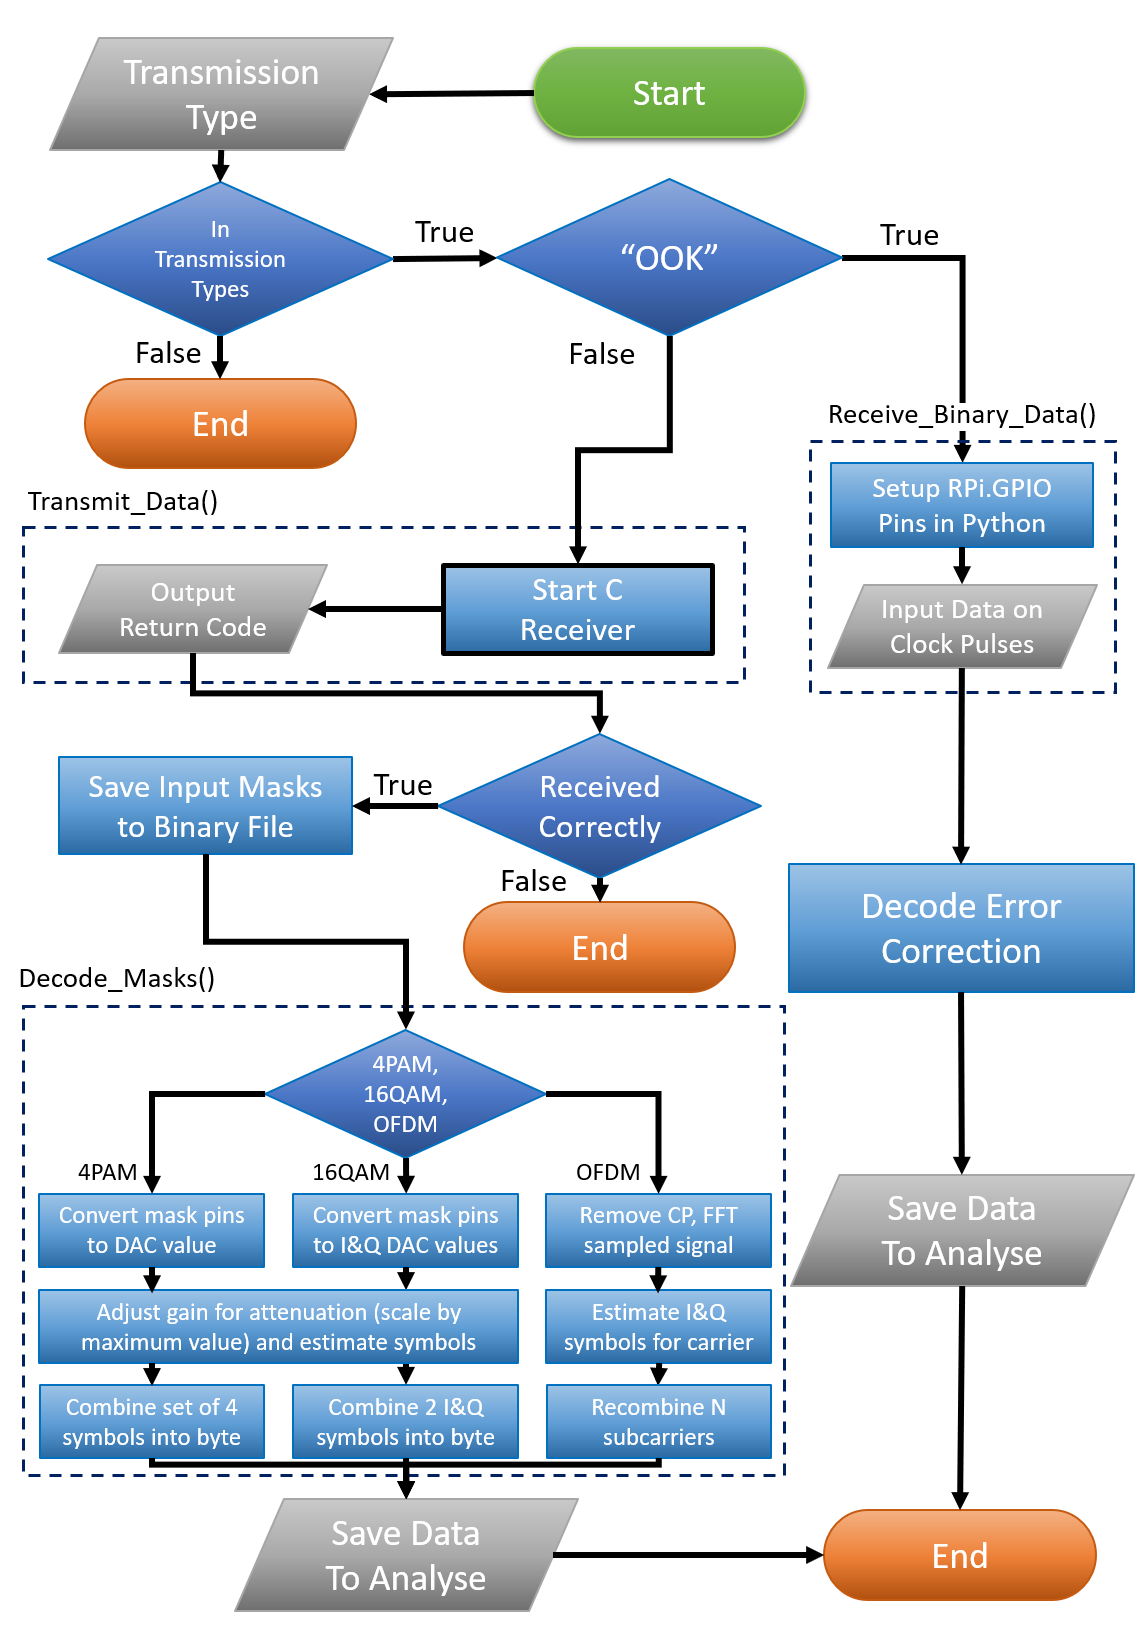
\includegraphics[width=\textwidth]{Receiver_Flow.png}
	\caption{Flow Chart for Receiver Code}
	\label{fig_Receiver_Flow}
\end{figure}

\subsubsection{Data and Image Handling}

NumPy and imageio.\\

\subsubsection{C Transmitter and Receiver}

Receiver: in Section \ref{sec_Computation} the options of data mask in on trigger vs read data then in on clock were compared and BLA was chosen as the more effective method.
\todo[inline]{Which method is more effective}

/* PiTransmit now works independent of the choice of DAC pins.
* It reads in the bit-mask (bits to set) from a binary file for speed,
* which is calculated and saved in the Python before transmission,
* and it also reads in inversion mask (bits to clear) so the calculation
* isn't done during transmission.
* This also means the Transmit program doesn't need to know how many
* DAC's there are so works for all transmission schemes.
*/

The pins selected are based on the DAC1 choice from Figure \ref{fig_Pin Connections} but could be used for any set of possible output pins.
\todo[inline,color=blue!20]{Add a comment about the range of 2 to 28 not 0 to 32 in bank writing}

\begin{figure}[ht]
	\centering
	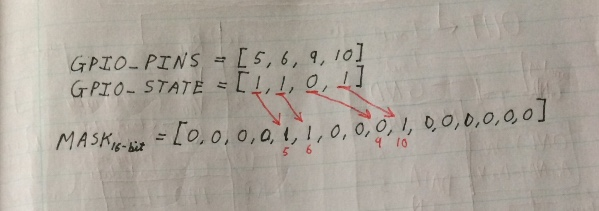
\includegraphics[width=0.6\textwidth]{Mask_Expansion.jpg}
	\caption{Explanation of the concept of mask expansion}
	%\label{fig_}
\end{figure}

\end{document}